\documentclass{beamer}
\usepackage[ngerman]{babel}
\usepackage[utf8]{inputenc}
%\usepackage[latin1]{inputenc}
\usepackage{amsmath}
\usepackage{amstext}
\usepackage{amssymb}
\usepackage{stmaryrd}
\usepackage{verbatim}
\usepackage{mathrsfs}

\usepackage{lmodern}

% Dadurch wird verhindert, dass die Navigationsleiste angezeigt wird.
%\setbeamertemplate{navigation symbols}{}

% zusaetzlich ist das usepackage{beamerthemeshadow} eingebunden 
\usepackage{beamerthemeshadow}

%  \beamersetuncovermixins{\opaqueness<1>{25}}{\opaqueness<2->{15}}
%  sorgt dafuer das die Elemente die erst noch (zukuenftig) kommen 
%  nur schwach angedeutet erscheinen 
\beamersetuncovermixins{\opaqueness<1>{25}}{\opaqueness<2->{15}}
% klappt auch bei Tabellen, wenn teTeX verwendet wird\ldots

\usetheme{Warsaw}  %% Themenwahl

\newcommand{\define}{\ensuremath{\mathrel{\mathop:}=}} % hübscheres :=, da = zentriert wird relativ zu :
\newcommand{\enifed}{\ensuremath{=\mathrel{\mathop:}}} % hübscheres =:, da = zentriert wird relativ zu :

%%%%%%%%%%%%%%%%%%%%%%%%%   Hoch minus Zahl
\newcommand{\1}{^{-1}}				
\newcommand{\2}{^{-2}}
\newcommand{\3}{^{-3}}
\newcommand{\4}{^{-4}}
\newcommand{\5}{^{-5}}
\newcommand{\6}{^{-6}}
\newcommand{\7}{^{-7}}
\newcommand{\8}{^{-8}}
\newcommand{\9}{^{-9}}
%%%%%%%%%%%%%%%%%%%%%%%%%%%%%%%%%%%%%%%%%%%%%%%%%%%%%%%%%%%%%%%%%%%%%%%%%%%%%%%%%%Pfeile
\newcommand{\imp}{\Longrightarrow}			% Implikation nach rechts
\newcommand{\pim}{\Longleftarrow}				% Implikation nach links	
\newcommand{\nach}{\longrightarrow}			% Menge pfeil nach rechts Menge für Funktionen
\newcommand{\hcan}{\longleftarrow}				% Menge pfeil nach links Menge für Funktionen
\newcommand{\nachmenge}{\longmapsto}		% x abgebildet auf f(x)
\newcommand{\aq}{\Longleftrightarrow}			% äquivalenz
\newcommand{\surj}{\twoheadrightarrow}		% surjektiver Pfeil nach rechts
\newcommand{\jrus}{\twoheadleftarrow}			% surjektiver Pfeil nach links
\newcommand{\inj}{\hookrightarrow}				% injektiver Pfeil nach rechts
\newcommand{\jni}{\hookleftarrow}				% injektiver Pfeil nach links
\newcommand{\ximp}{\xLongrightarrow}			%  \xLongrightarrow[\text{unten Text}]{\text{oben Text}} 
																		%%%% Implikation Text oben und untern 
\newcommand{\xpim}{\xLongleftarrow}
																		%  \xLeftrightarrow[\text{unten Text}]{\text{oben Text}} 
																		%%%% Äquivalenz Text oben und unten
\newcommand{\xaq}{\xLeftrightarrow}	
																		%%%% Menge nach Menge mit text über und unter Pfeil
\newcommand{\xnach}{\xlongrightarrow}		
\newcommand{\xhcan}{\xlongleftarrow}										

\renewcommand{\l}{\left\vert}   						%linker Betragsstrich
\renewcommand{\r}{\right\vert}						%rechter Betragsstrich
\newcommand{\ecap}{\cap \ldots \cap}			%Schnit ... Schnitt
\newcommand{\ecup}{\cup \ldots \cup}			%Vereinigung ... Vereinigung
\newcommand{\eplus}{+ \ldots +}					% + ... +
\newcommand{\ekomma}{{,} \ldots {,}}			% , ... ,
\newcommand{\x}{\times}								%  kreuz 
\renewcommand{\tilde}{\widetilde}
%%%%%%%%%%%%%%%%%%%%%%%%%%%% Bestimmte Mengen 
\newcommand{\N}{\ensuremath{\mathbb{N}}}
\newcommand{\Q}{\ensuremath{\mathbb{Q}}}
\newcommand{\Z}{\ensuremath{\mathbb{Z}}}
\newcommand{\F}{\ensuremath{\mathbb{F}}}
\newcommand{\R}{\ensuremath{\mathbb{R}}}
\newcommand{\C}{\ensuremath{\mathbb{C}}}

\title{Präsentation zum Thema Meinungsdynamik}
\author{Gentian Rrafshi}
\date{\today}
 
\begin{document}

\begin{frame}
\titlepage
\end{frame} 

{
\usebackgroundtemplate{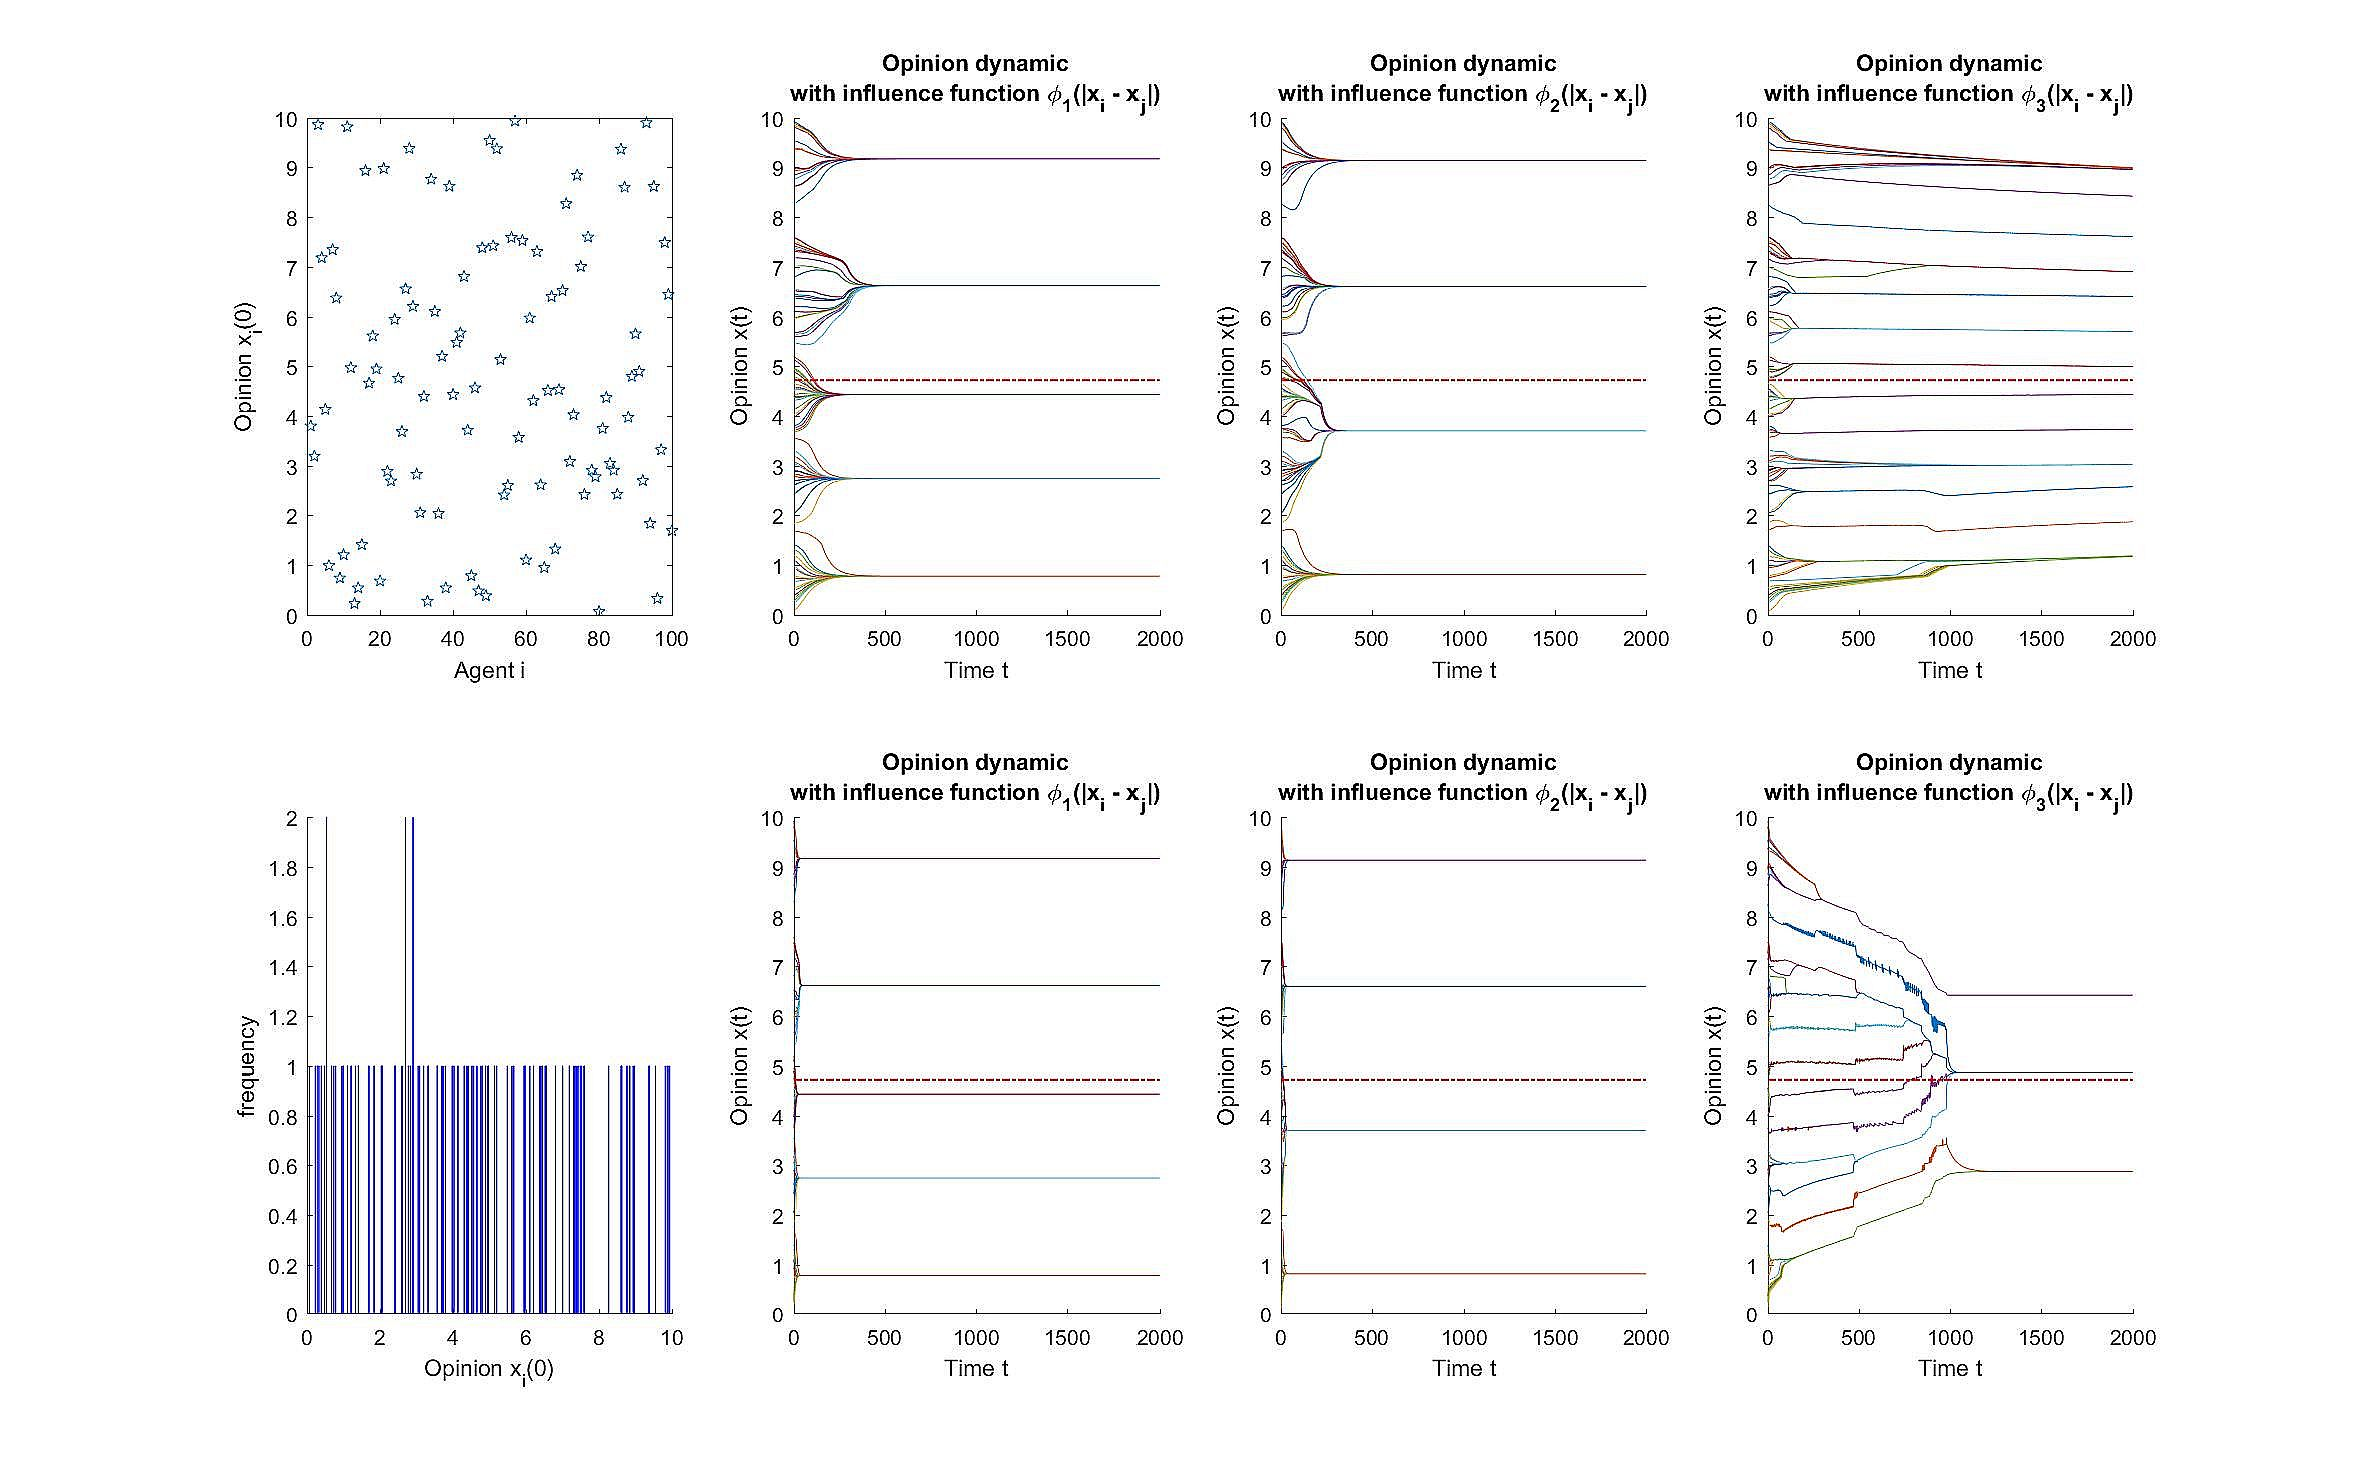
\includegraphics[width=\paperwidth , height=\paperheight]{0}}
\begin{frame}[plain]

\end{frame}
}

{
\usebackgroundtemplate{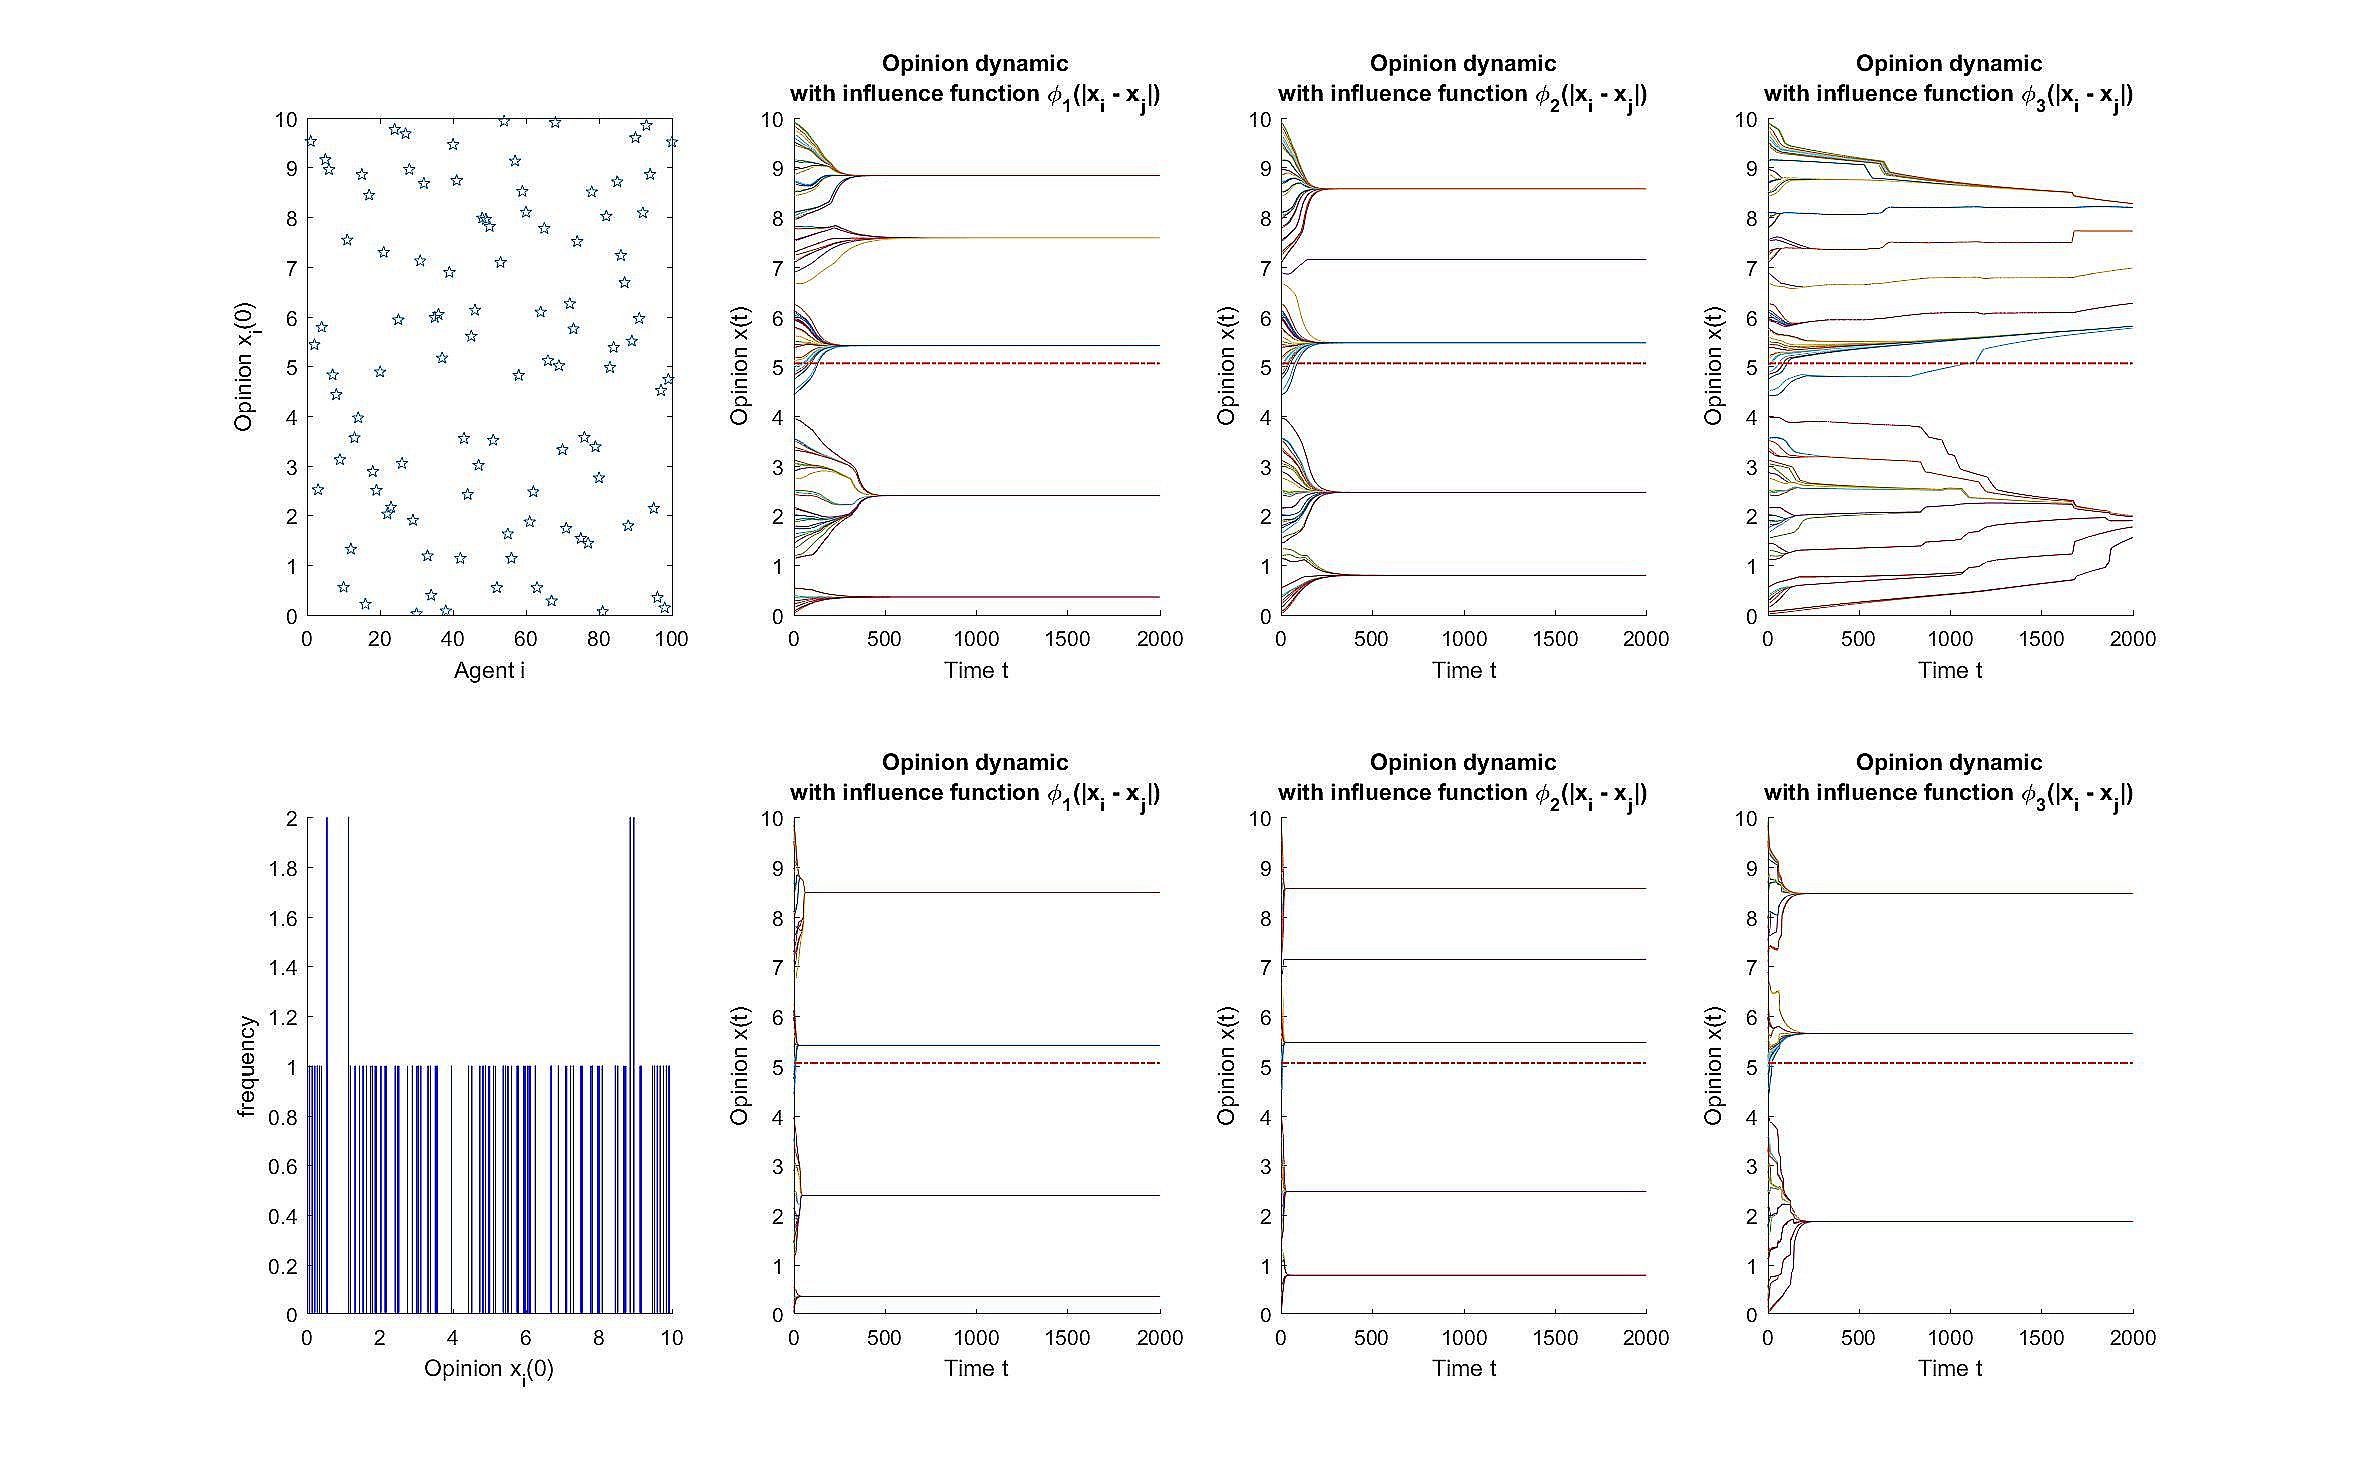
\includegraphics[width=\paperwidth , height=\paperheight]{1}}
\begin{frame}[plain]

\end{frame}
}

{
\usebackgroundtemplate{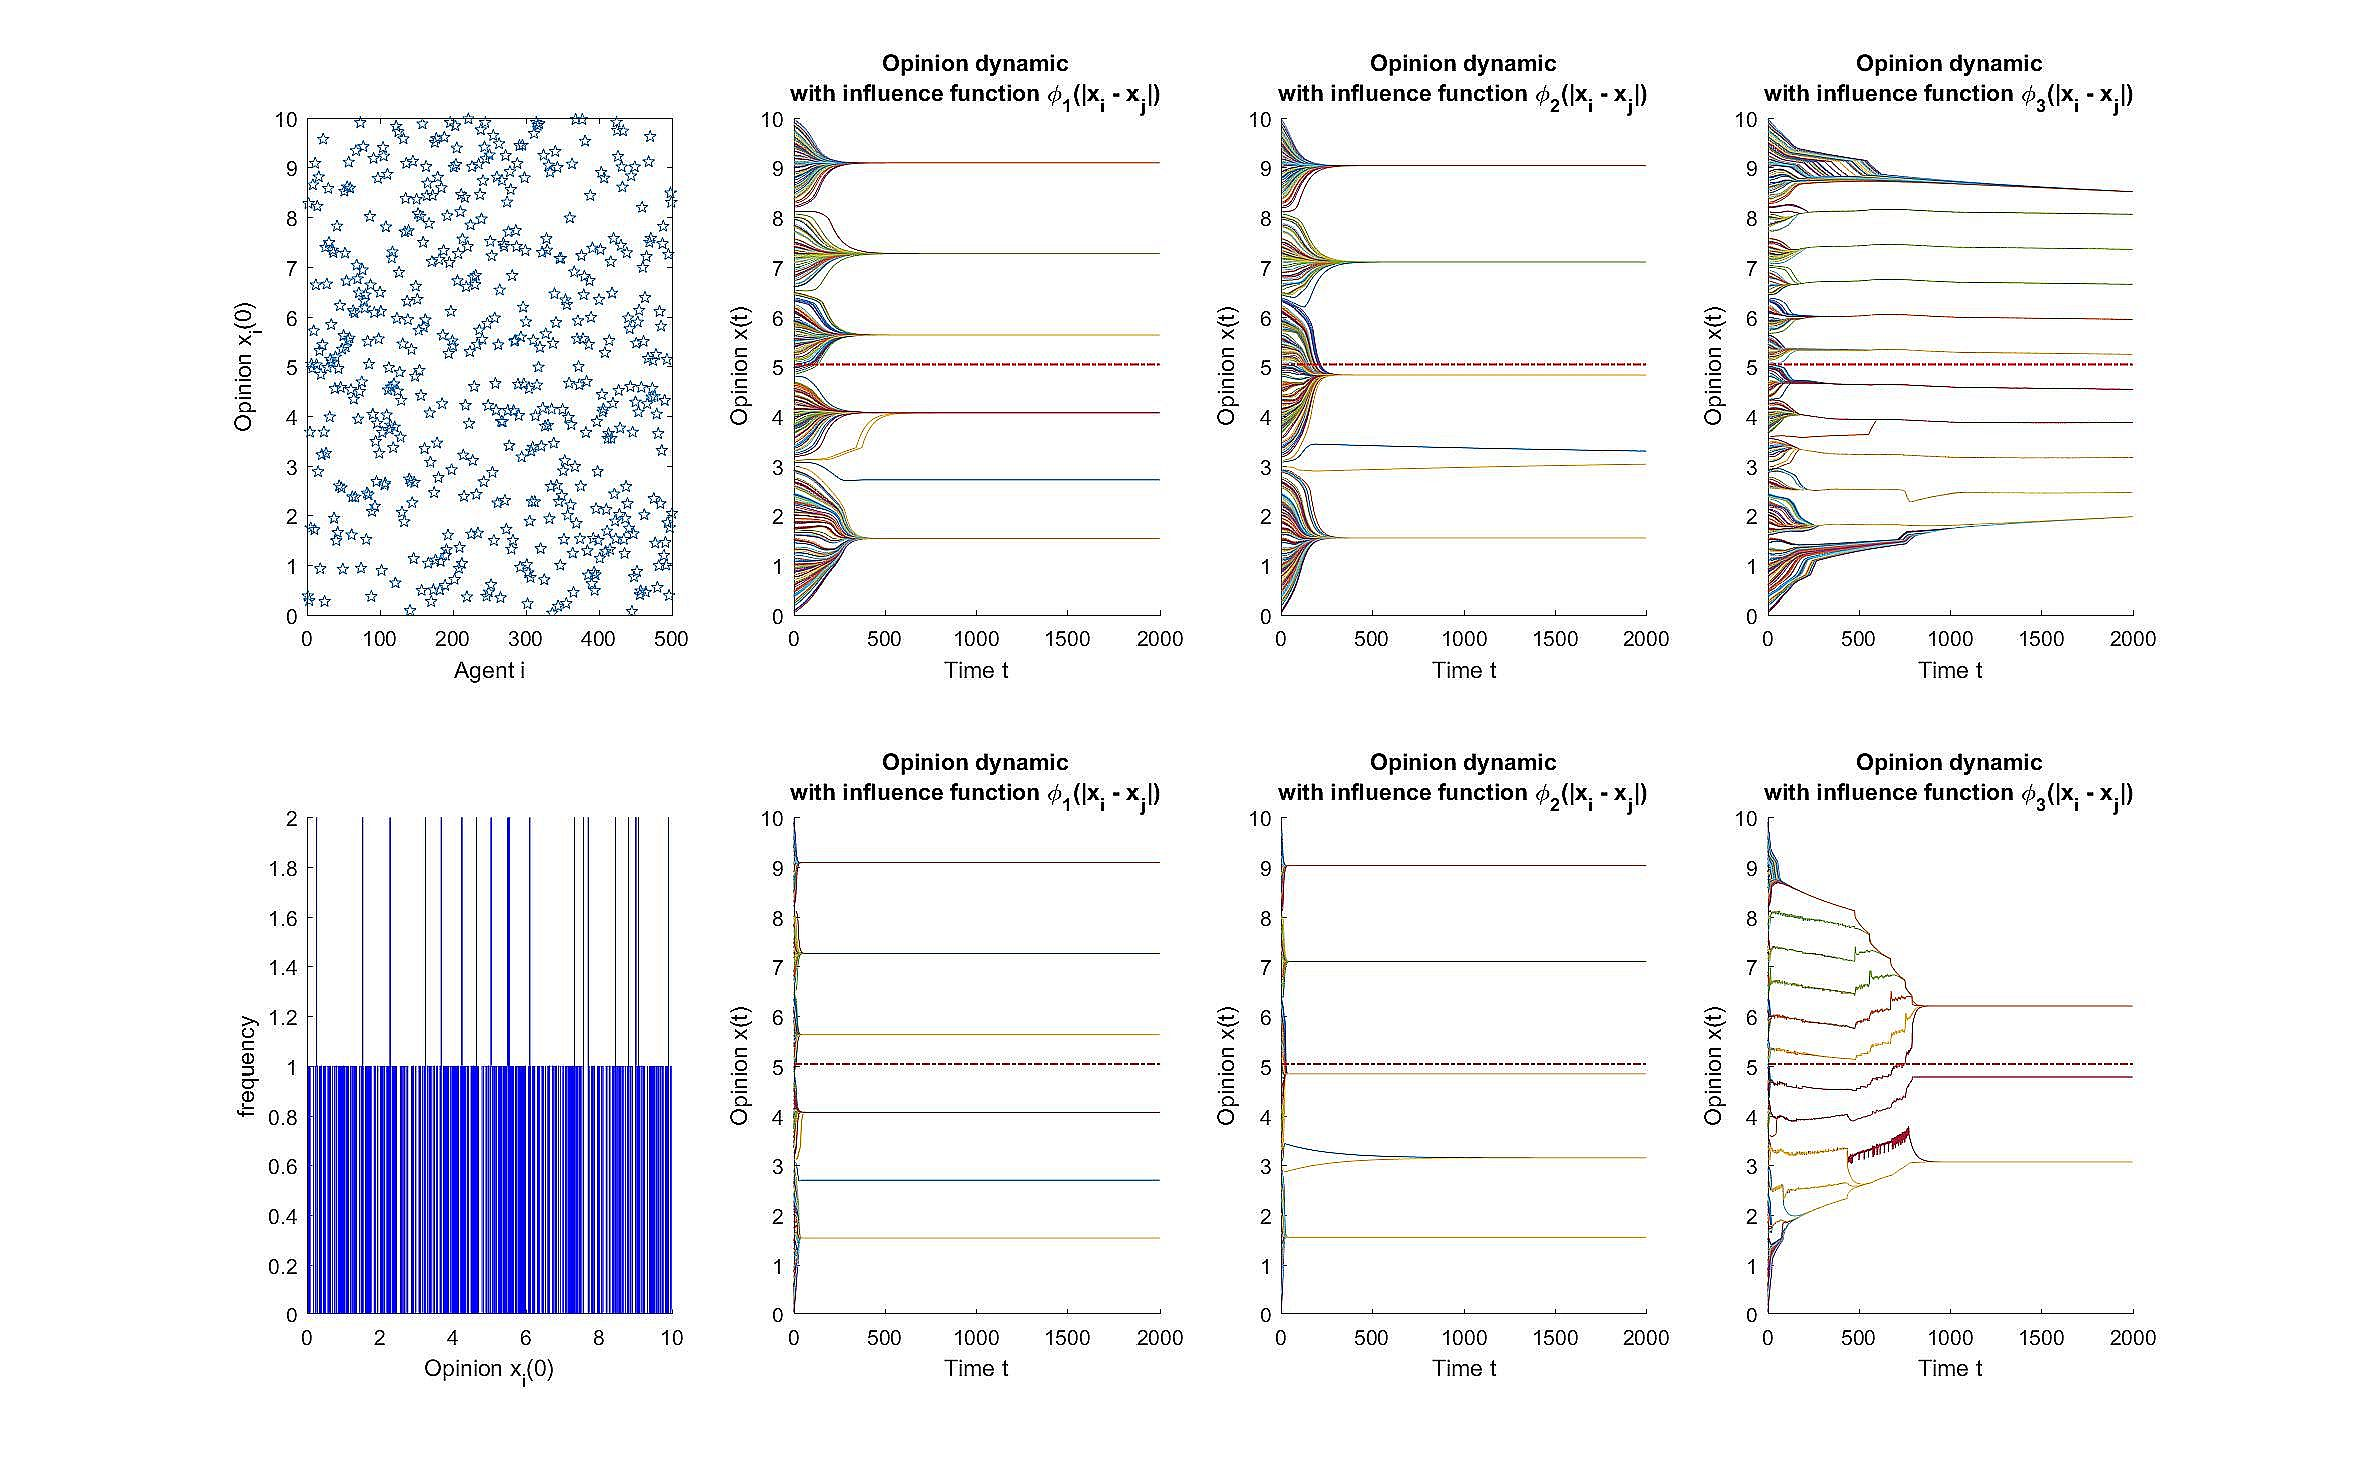
\includegraphics[width=\paperwidth , height=\paperheight]{2}}
\begin{frame}[plain]

\end{frame}
}

{
\usebackgroundtemplate{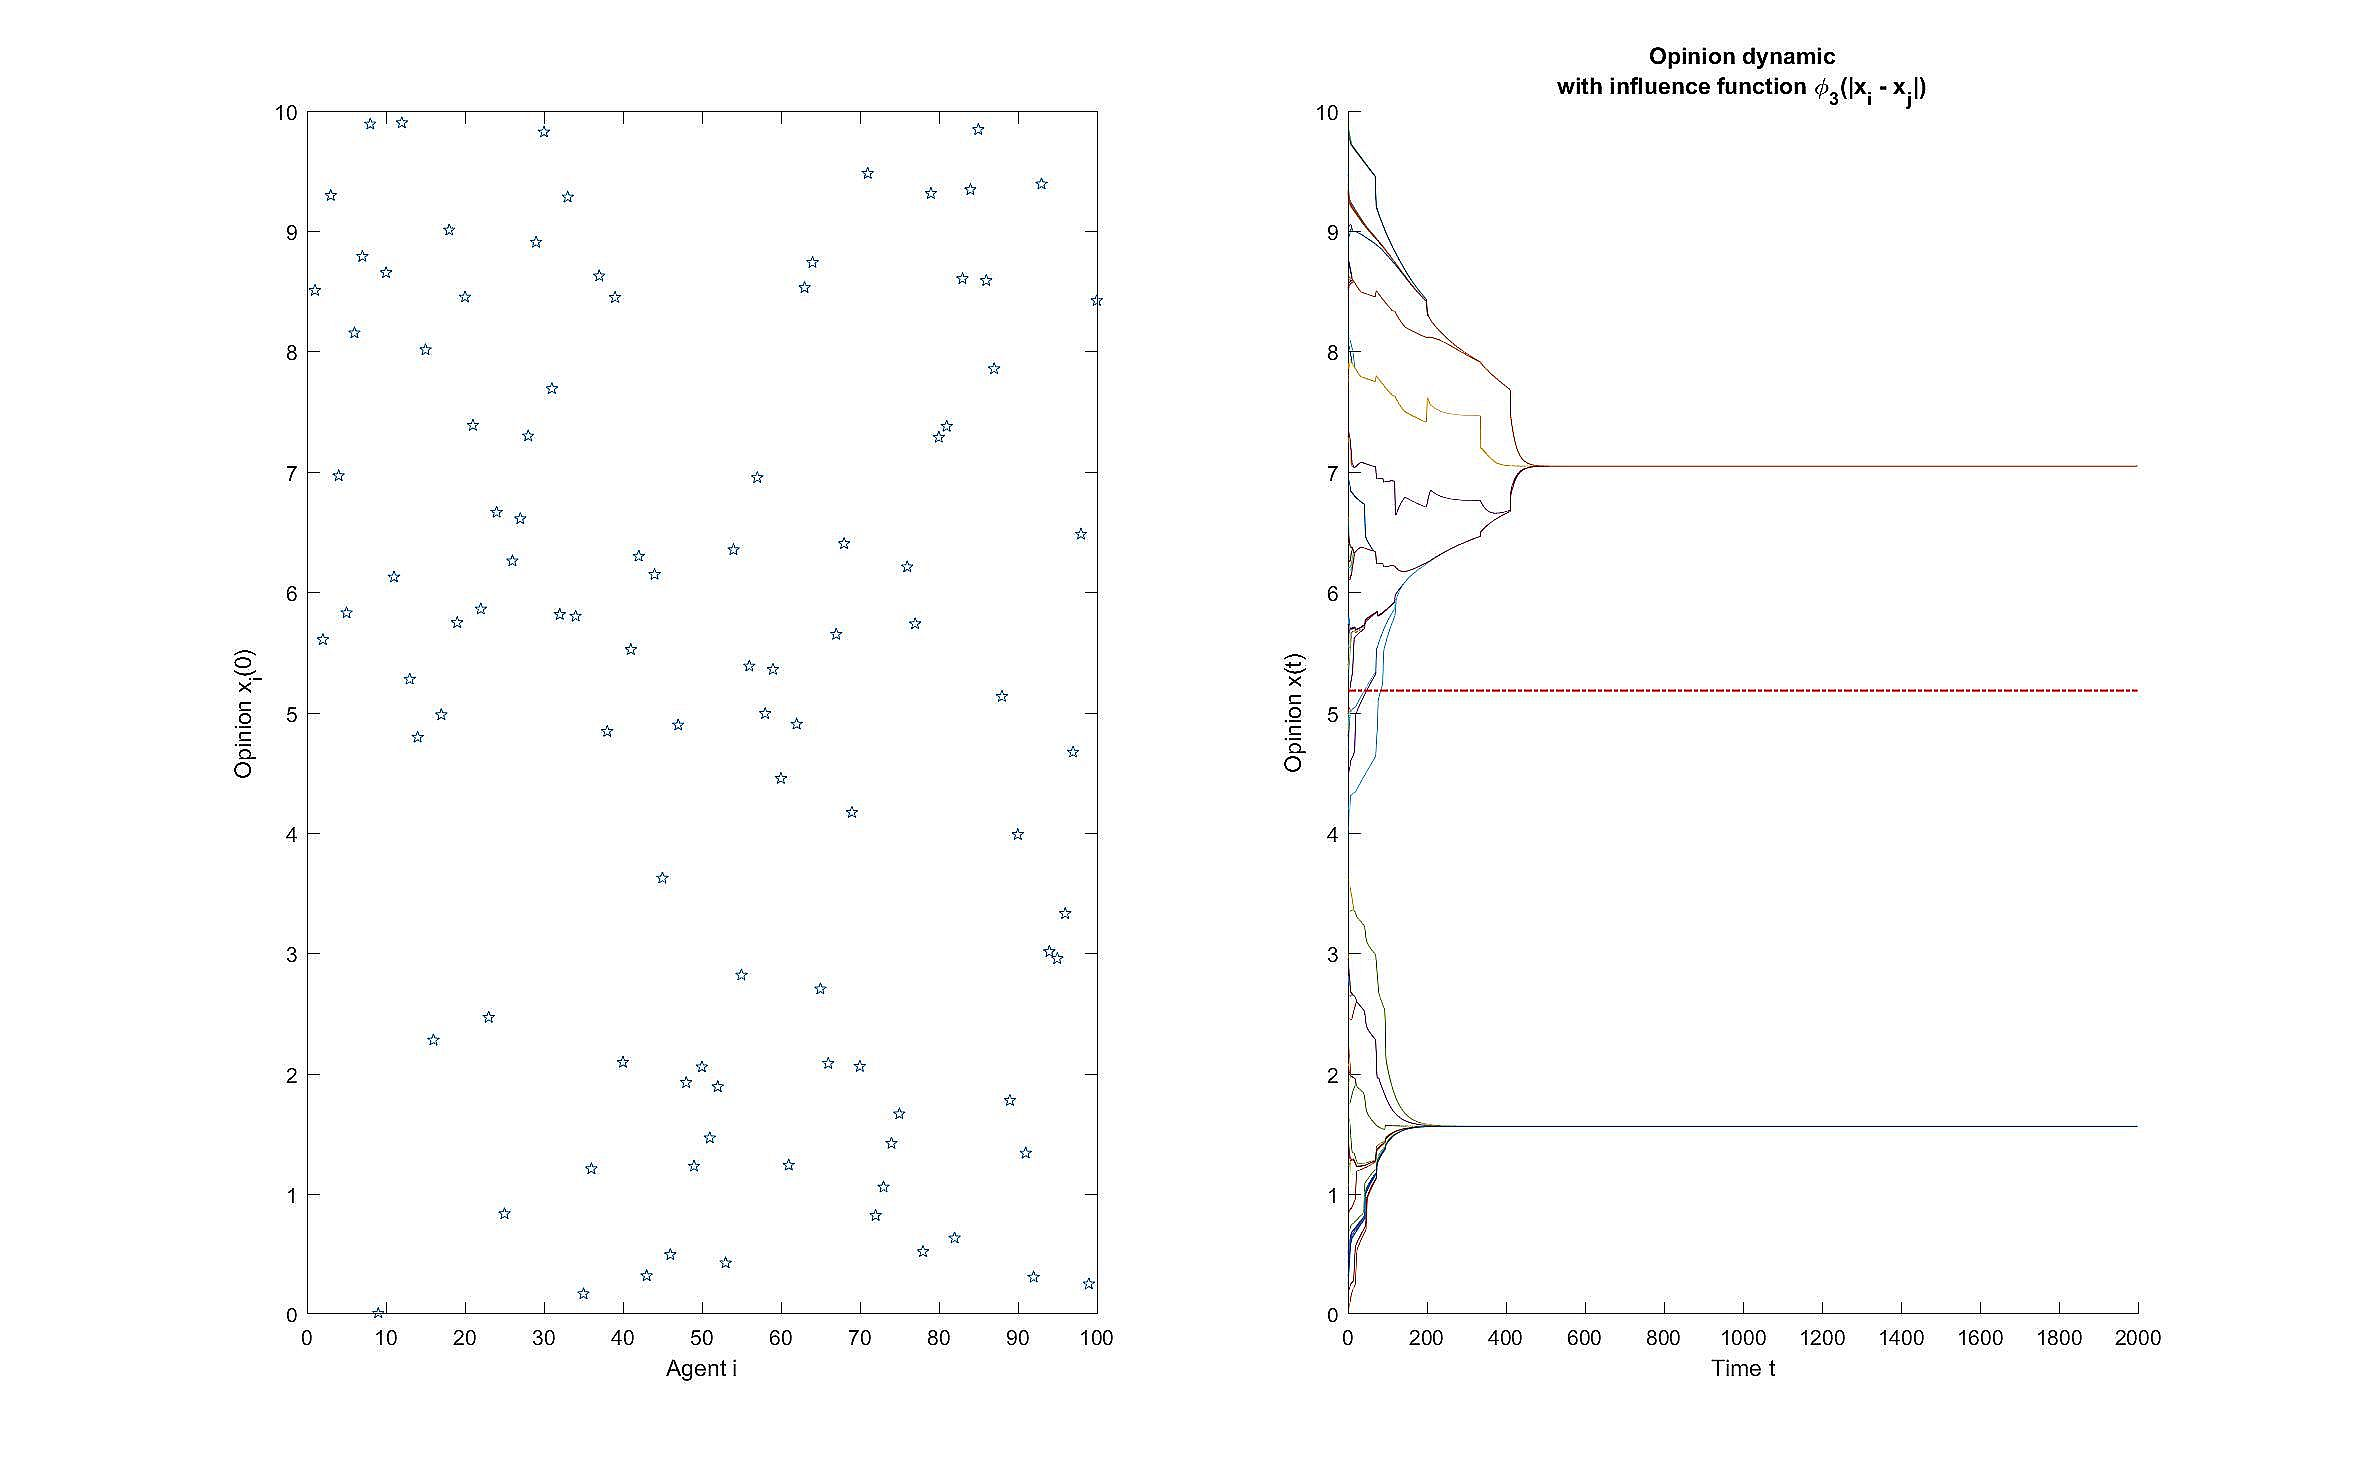
\includegraphics[width=\paperwidth , height=\paperheight]{3}}
\begin{frame}[plain]

\end{frame}
}

{
\usebackgroundtemplate{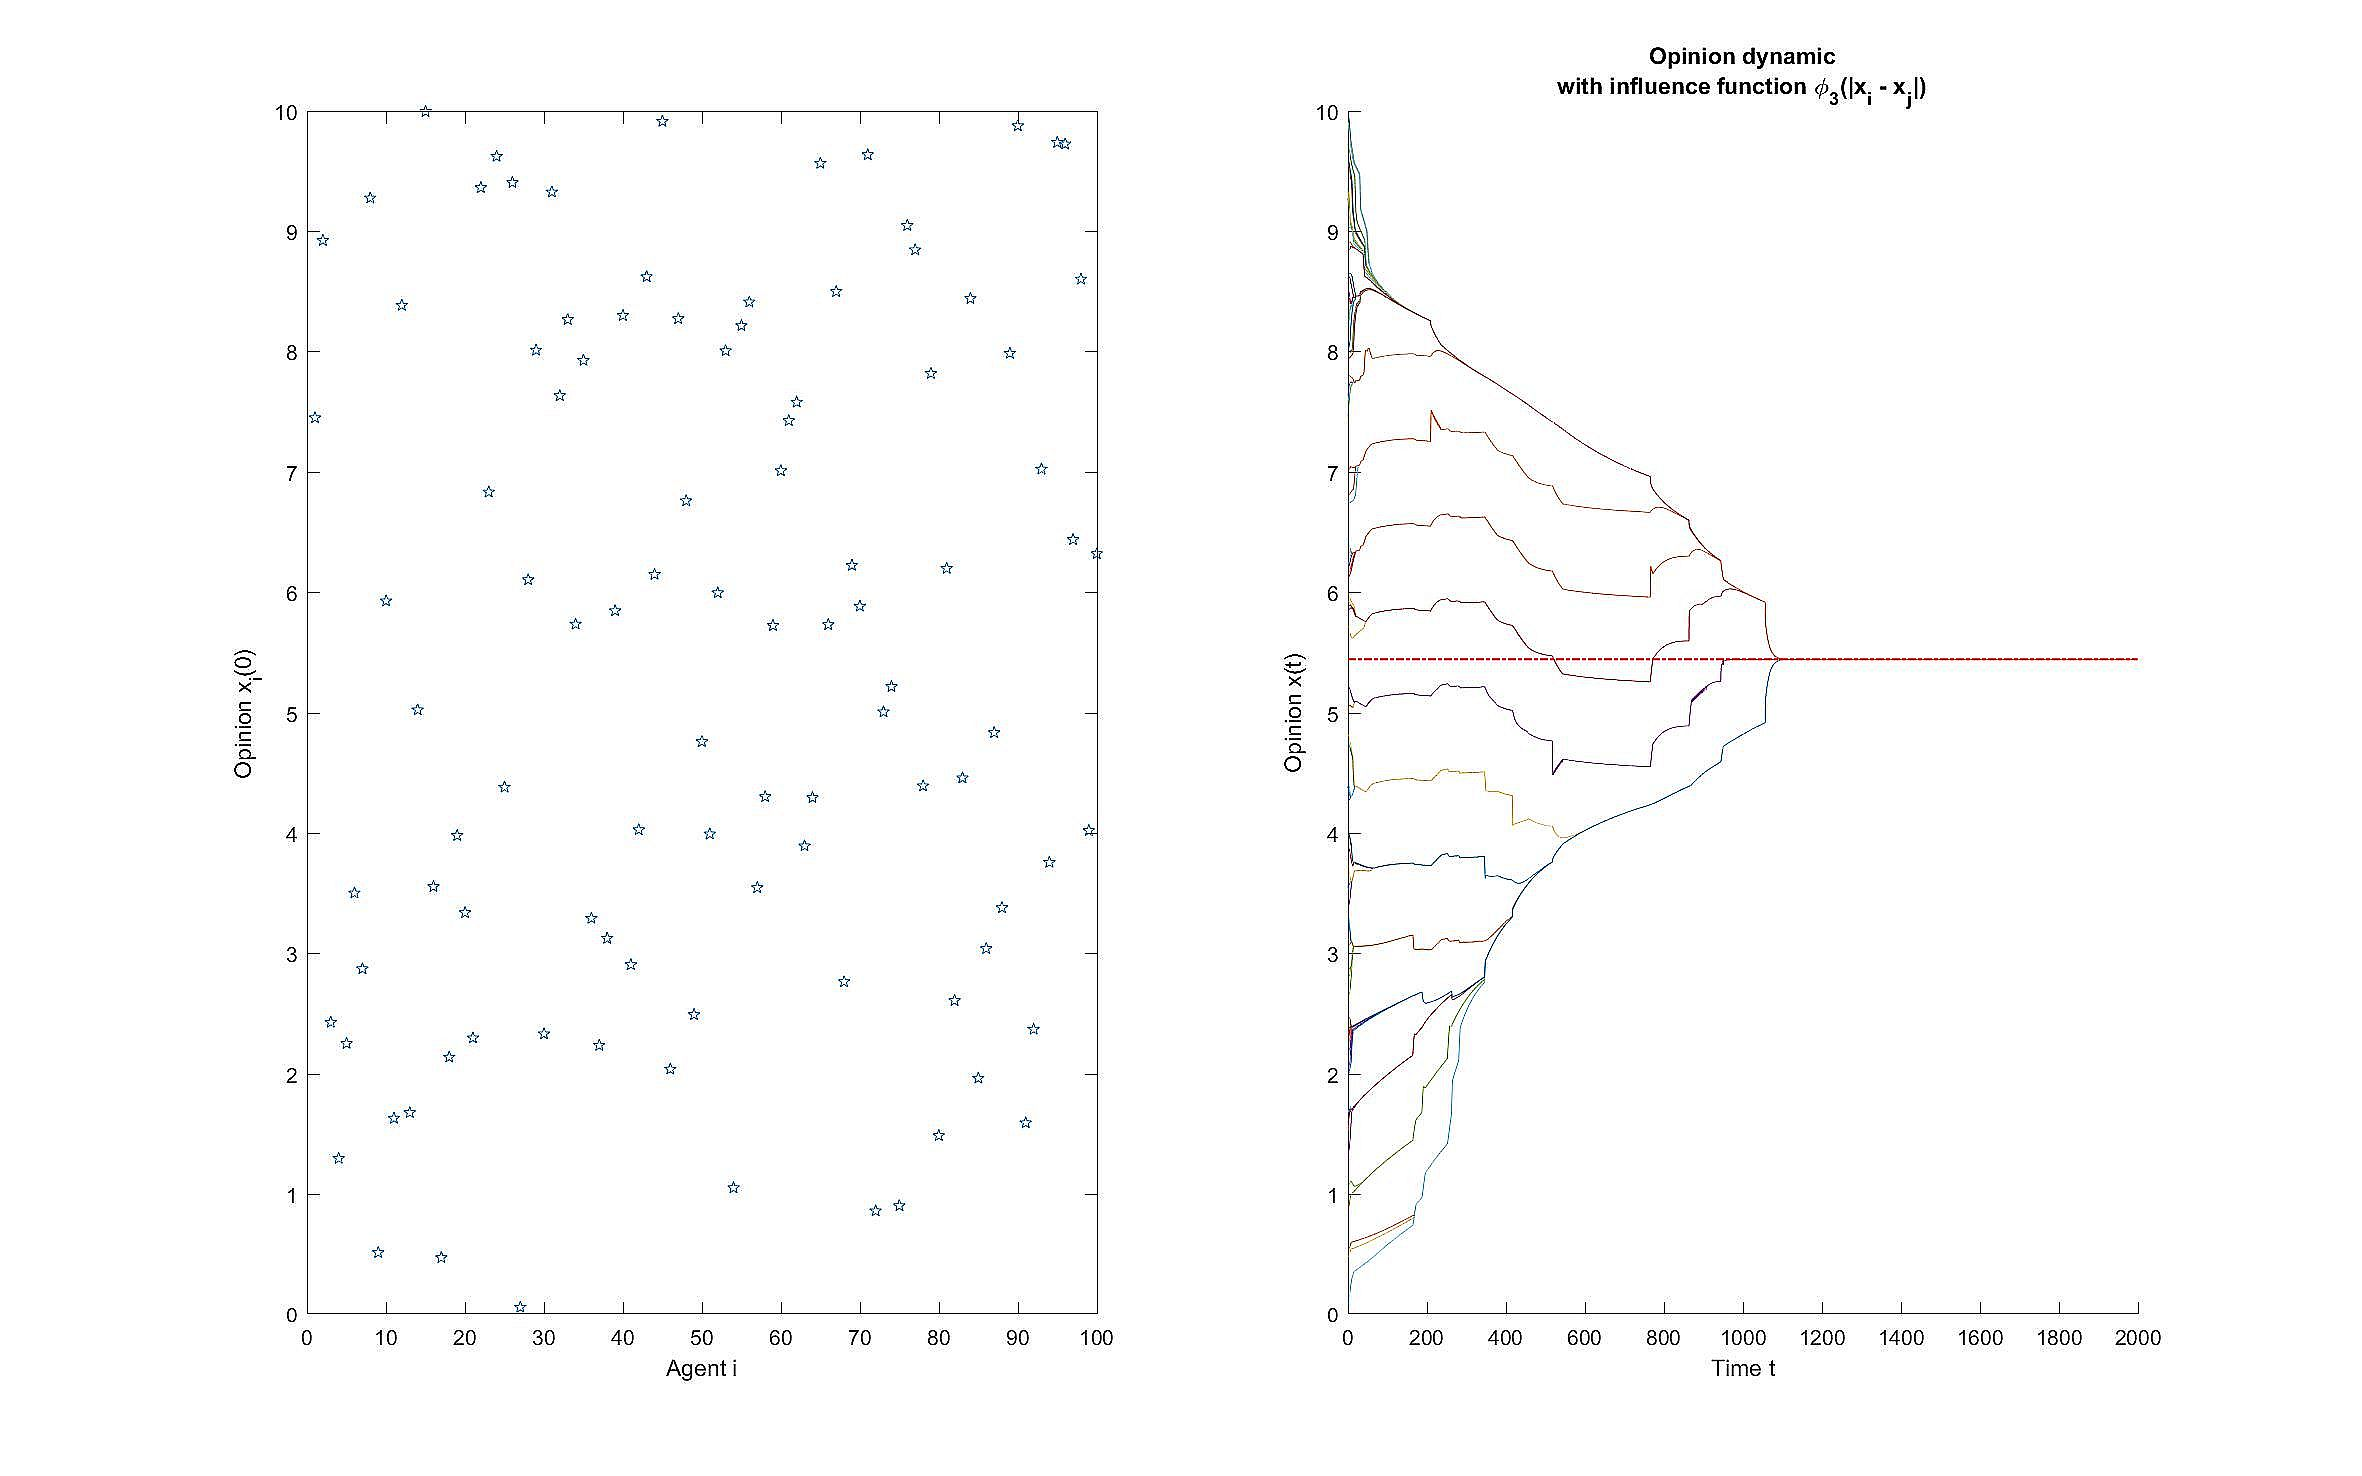
\includegraphics[width=\paperwidth , height=\paperheight]{4}}
\begin{frame}[plain]

\end{frame}
}

{
\usebackgroundtemplate{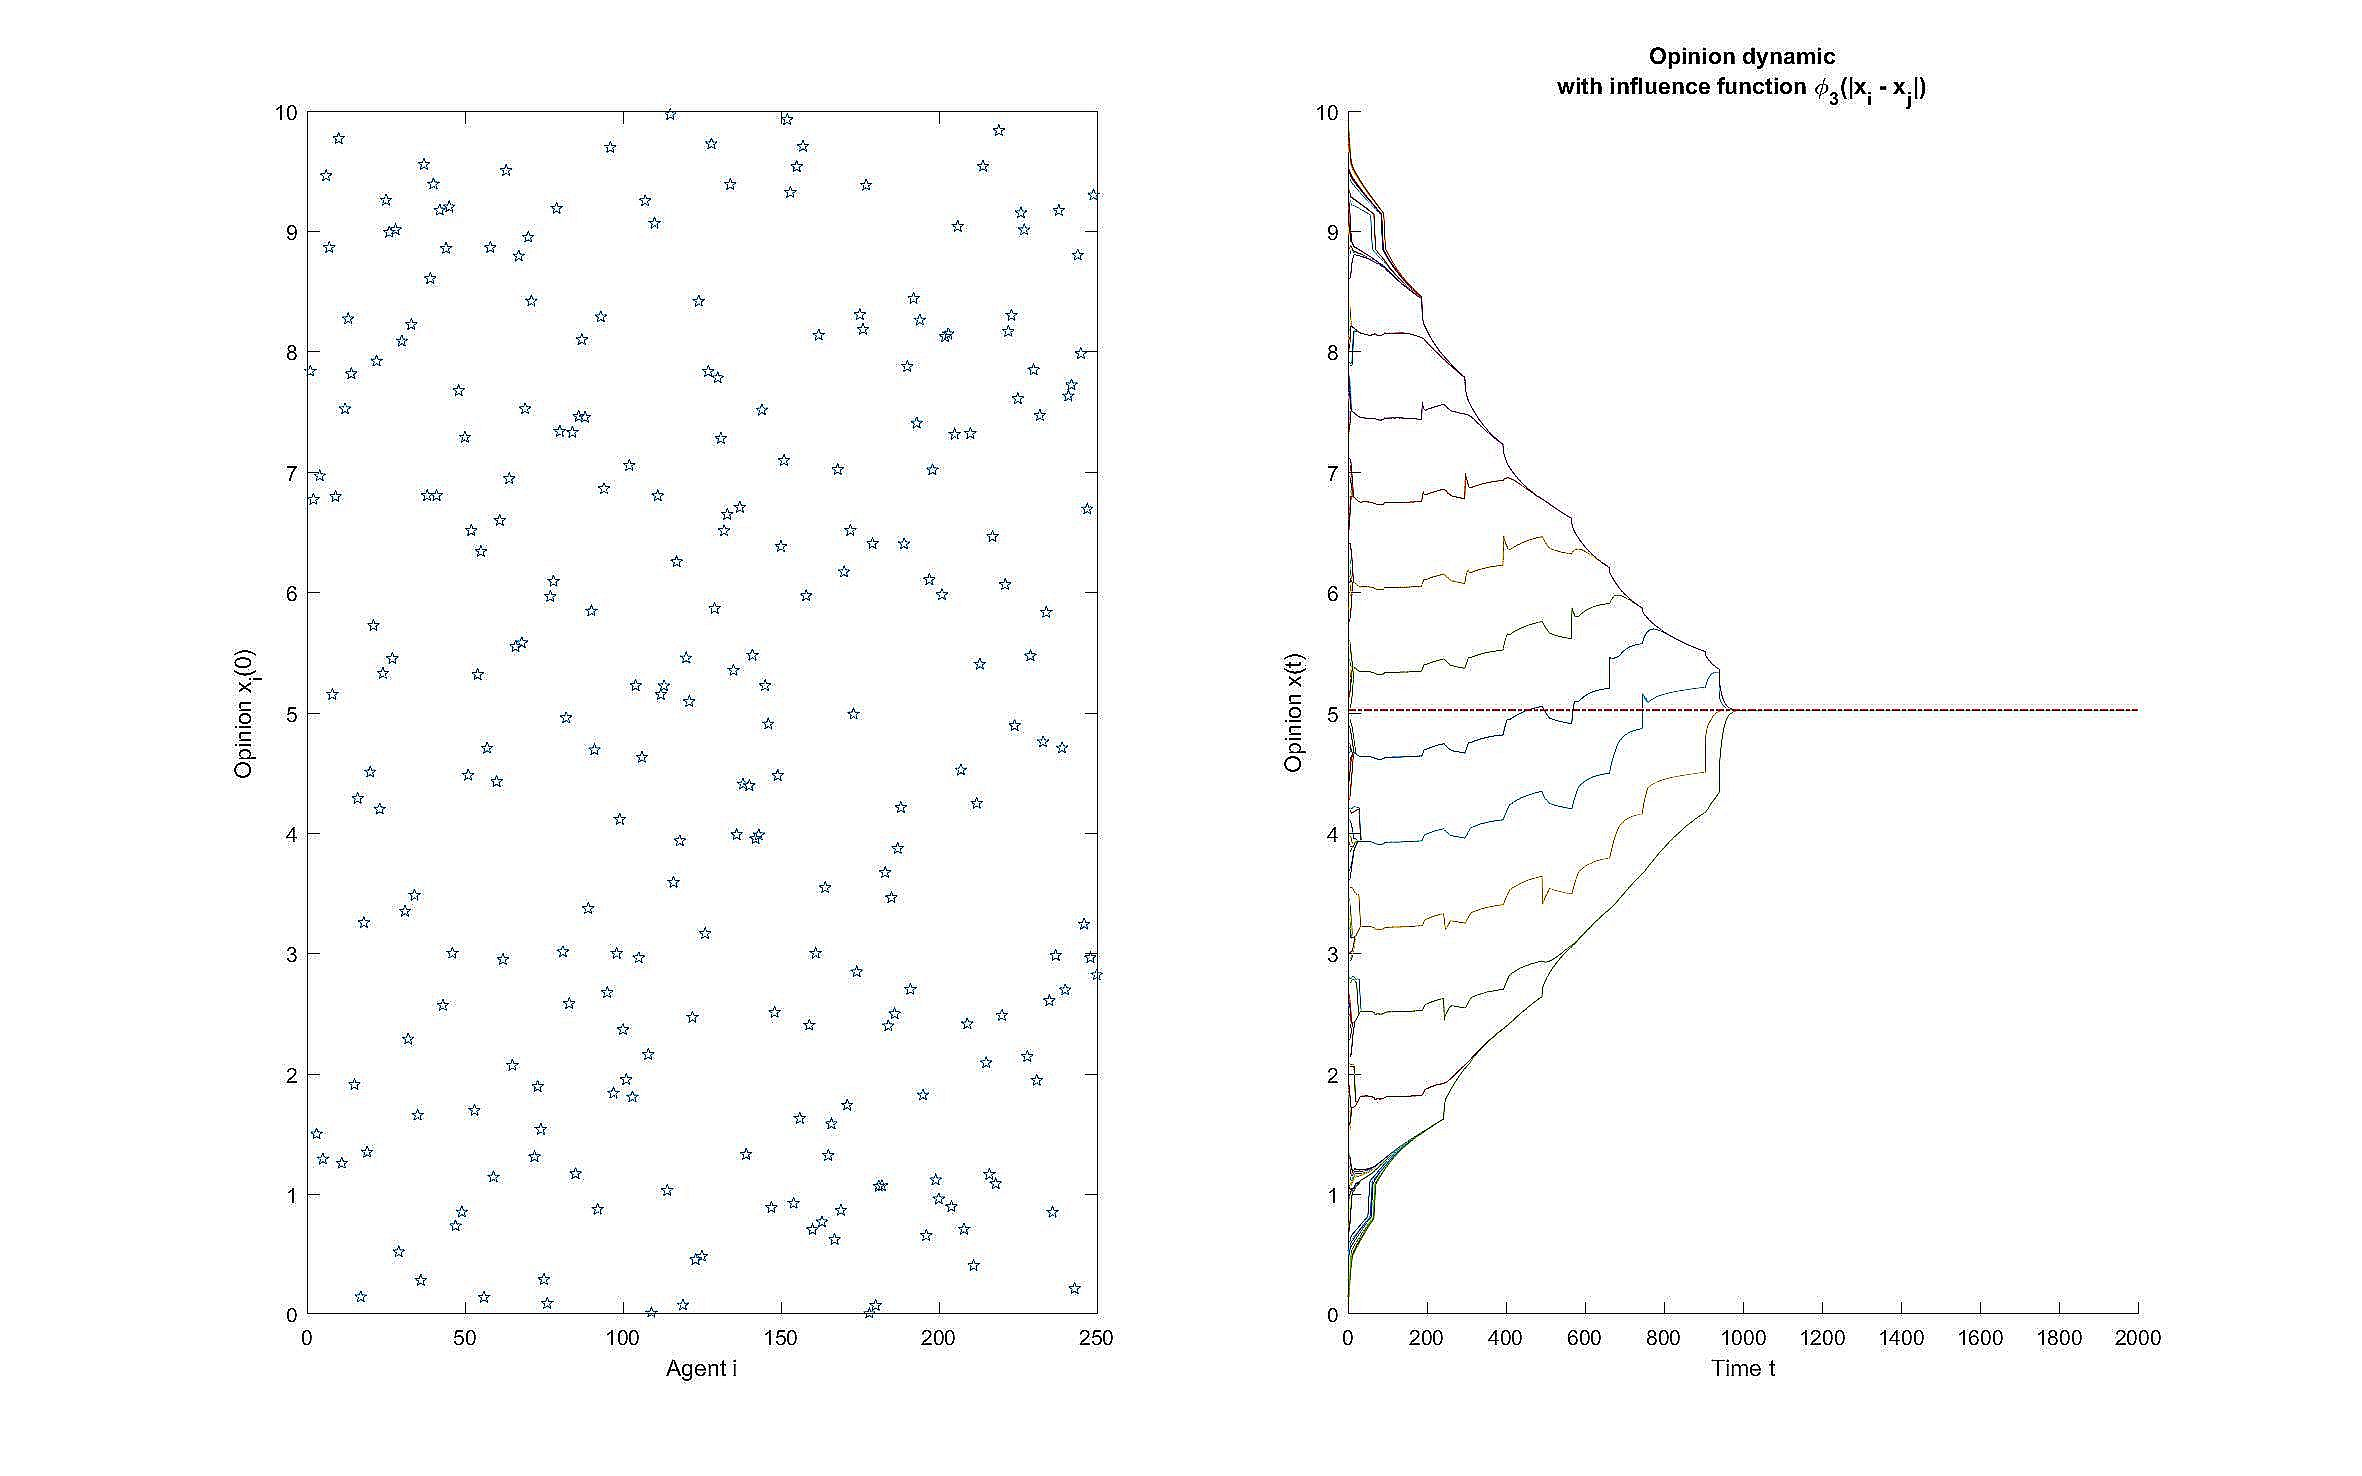
\includegraphics[width=\paperwidth , height=\paperheight]{5}}
\begin{frame}[plain]

\end{frame}
}

{
\usebackgroundtemplate{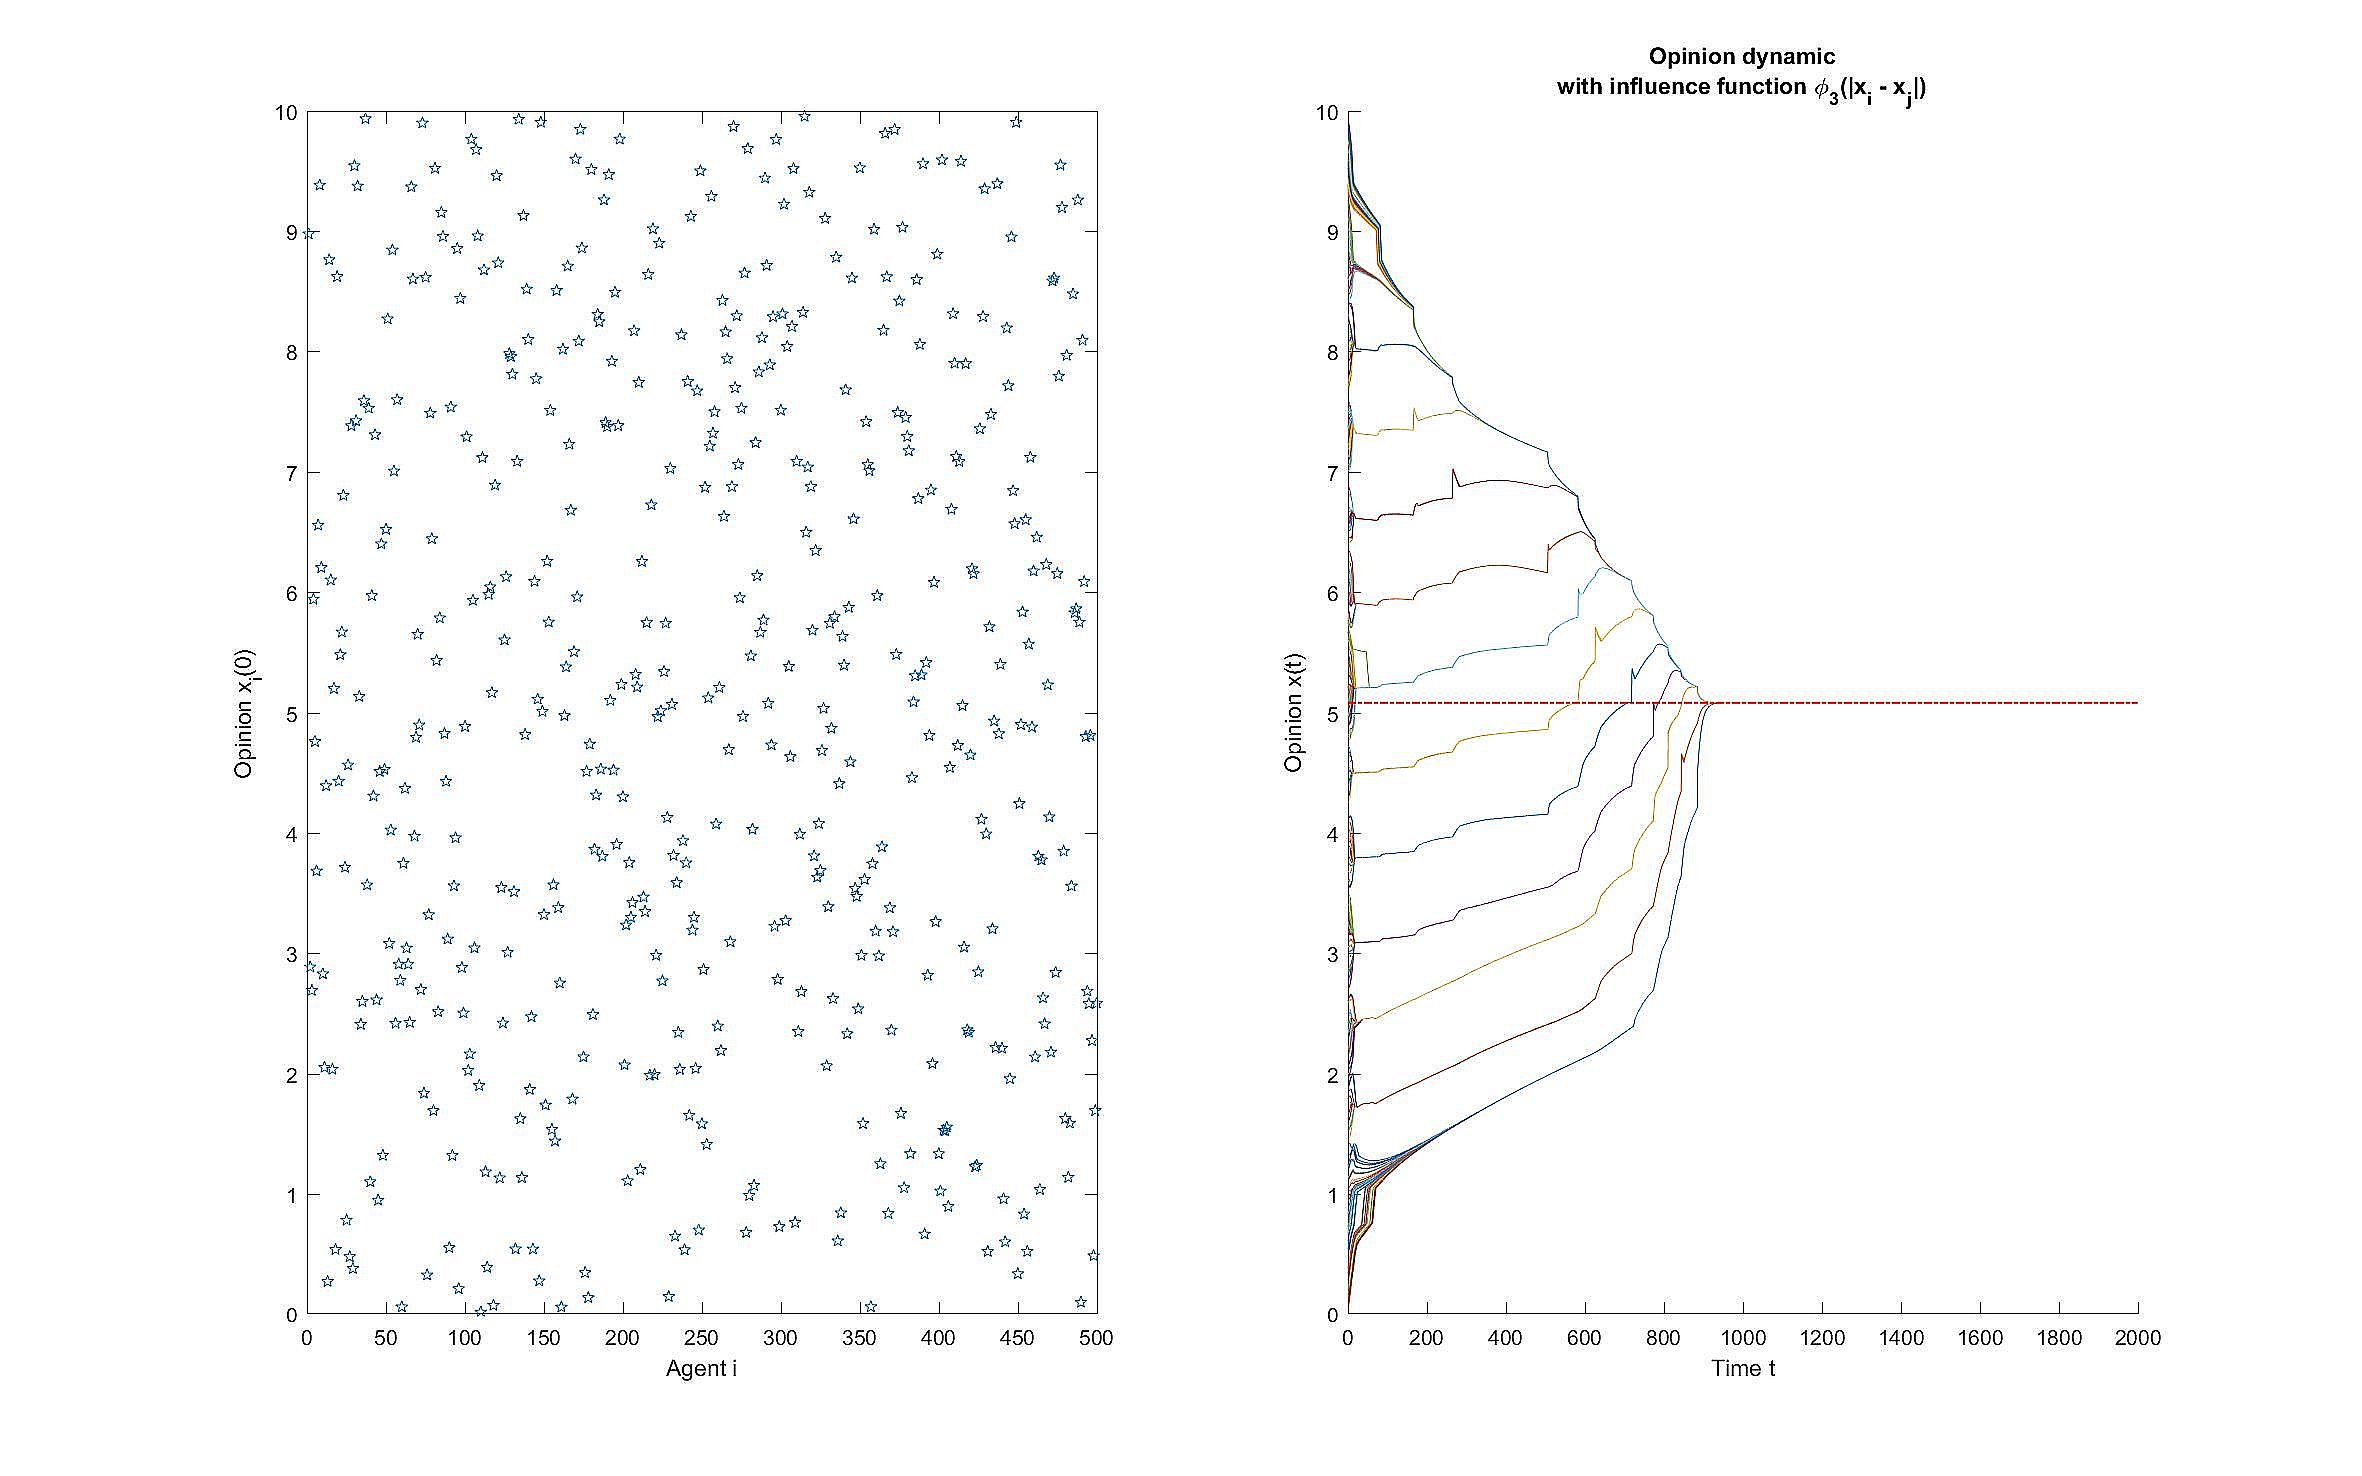
\includegraphics[width=\paperwidth , height=\paperheight]{6}}
\begin{frame}[plain]

\end{frame}
}

{
\usebackgroundtemplate{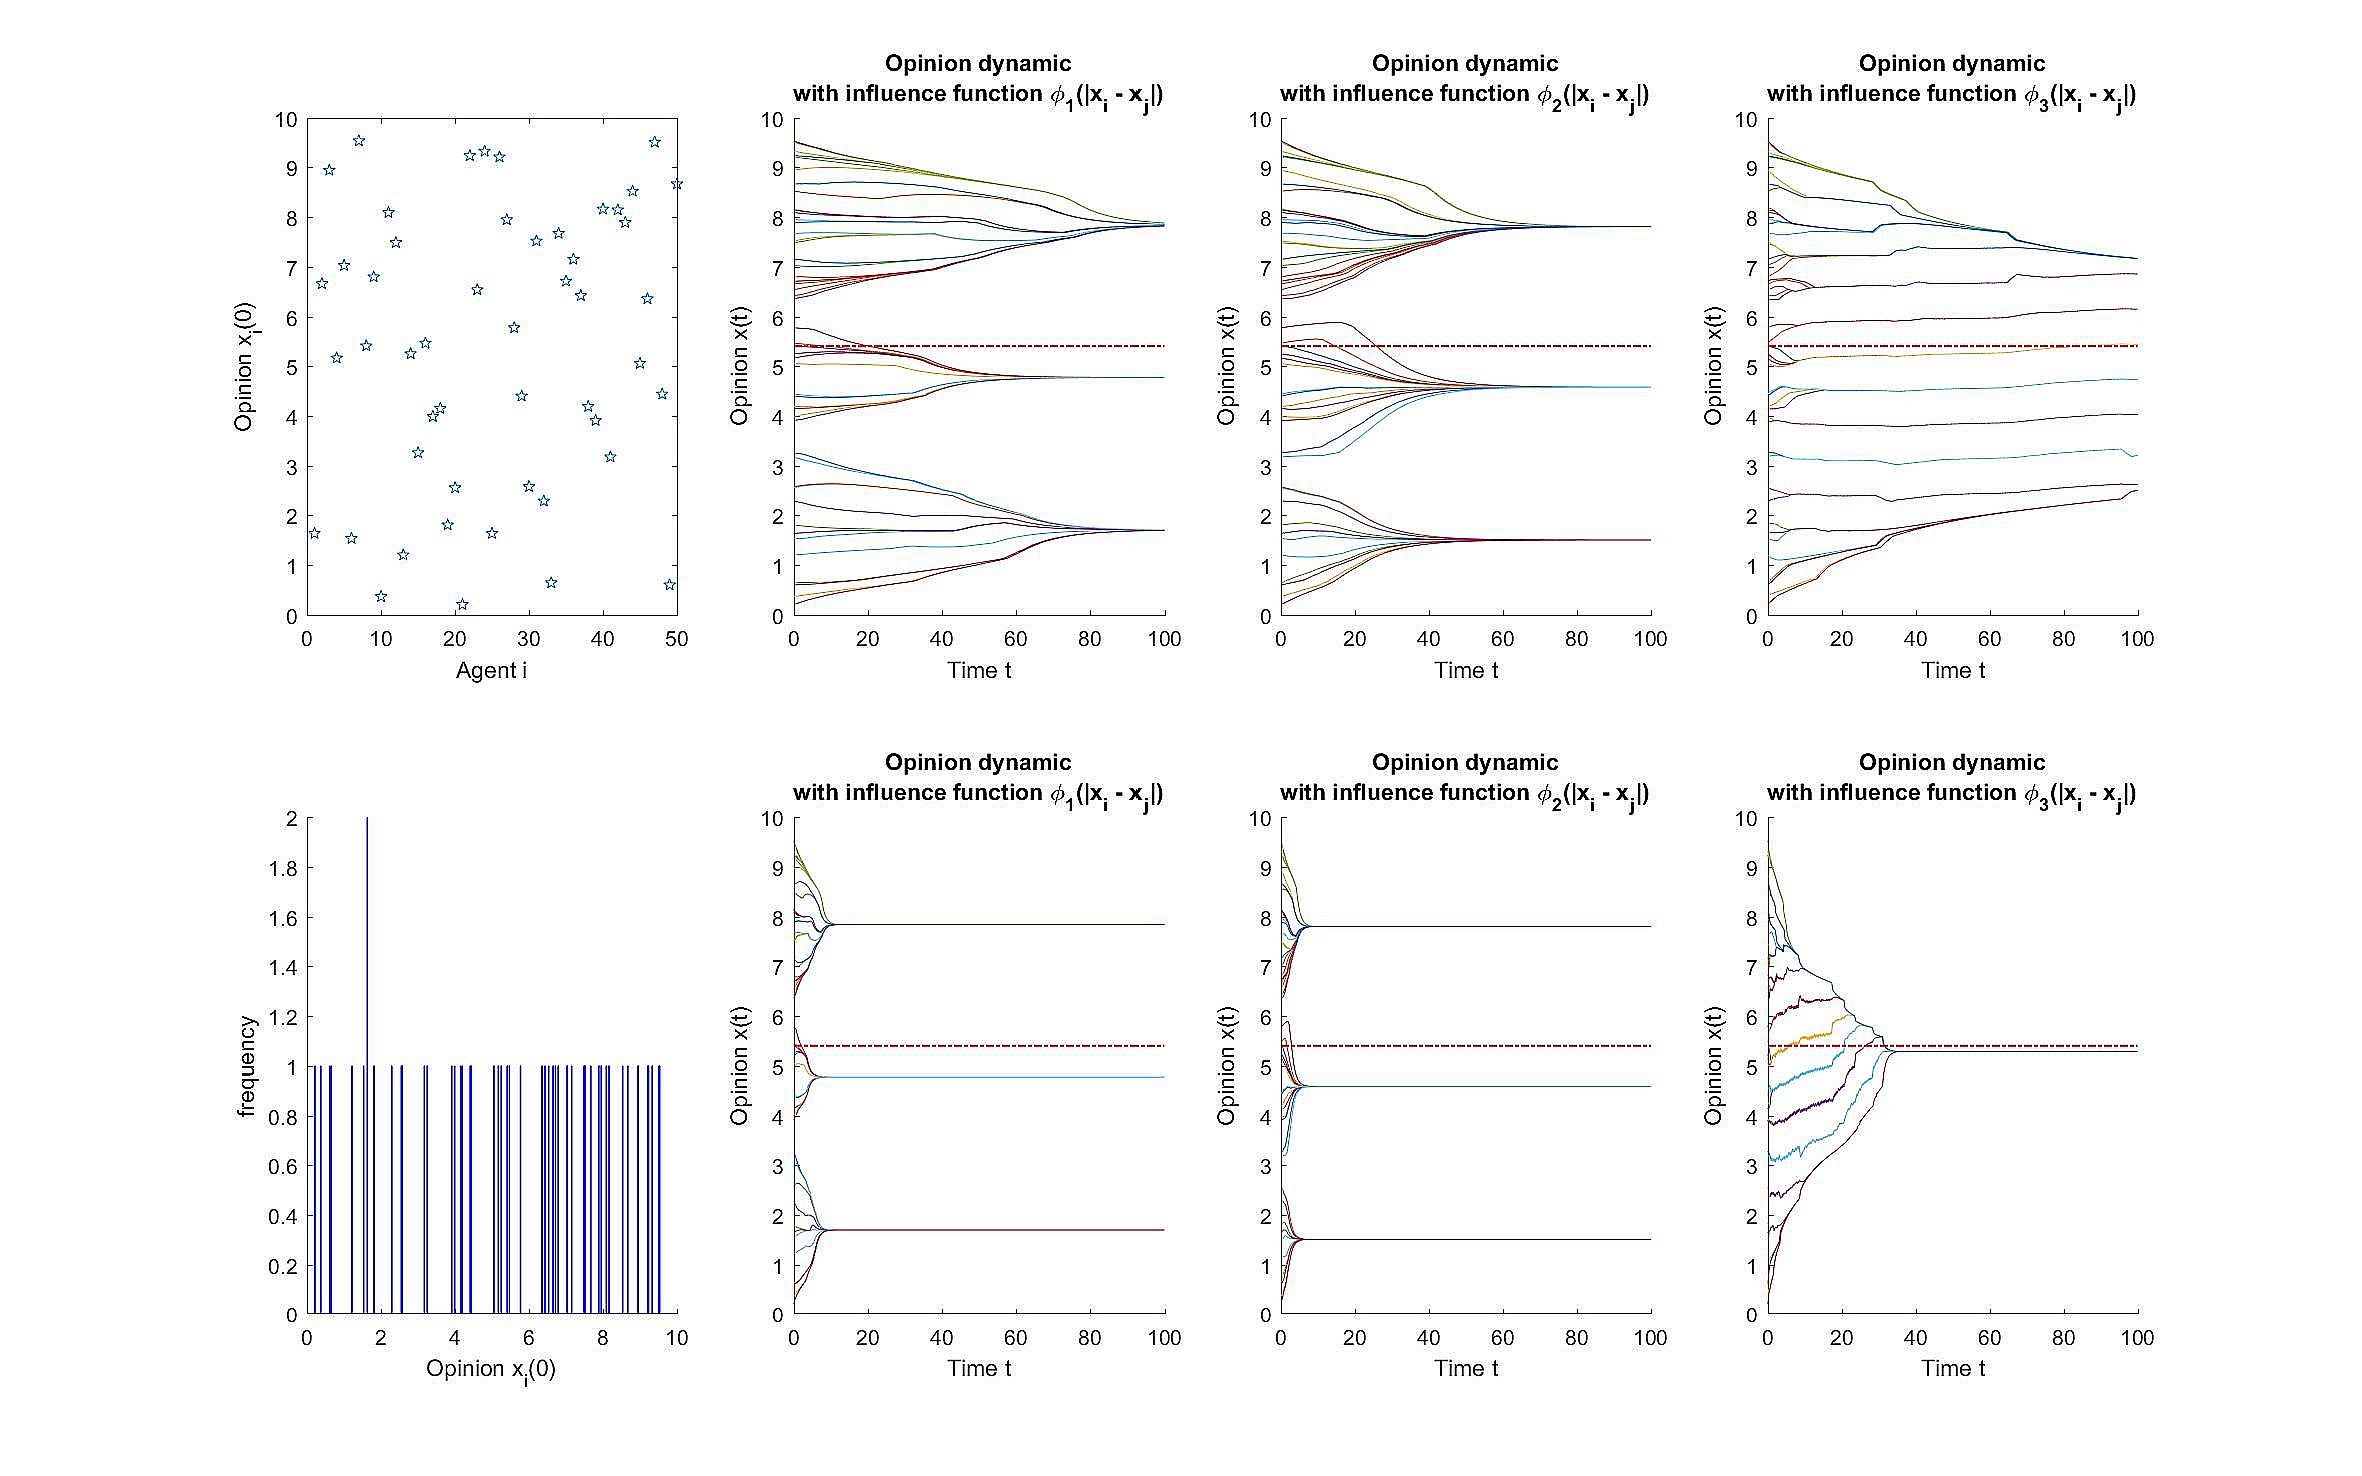
\includegraphics[width=\paperwidth , height=\paperheight]{7}}
\begin{frame}[plain]

\end{frame}
}

{
\usebackgroundtemplate{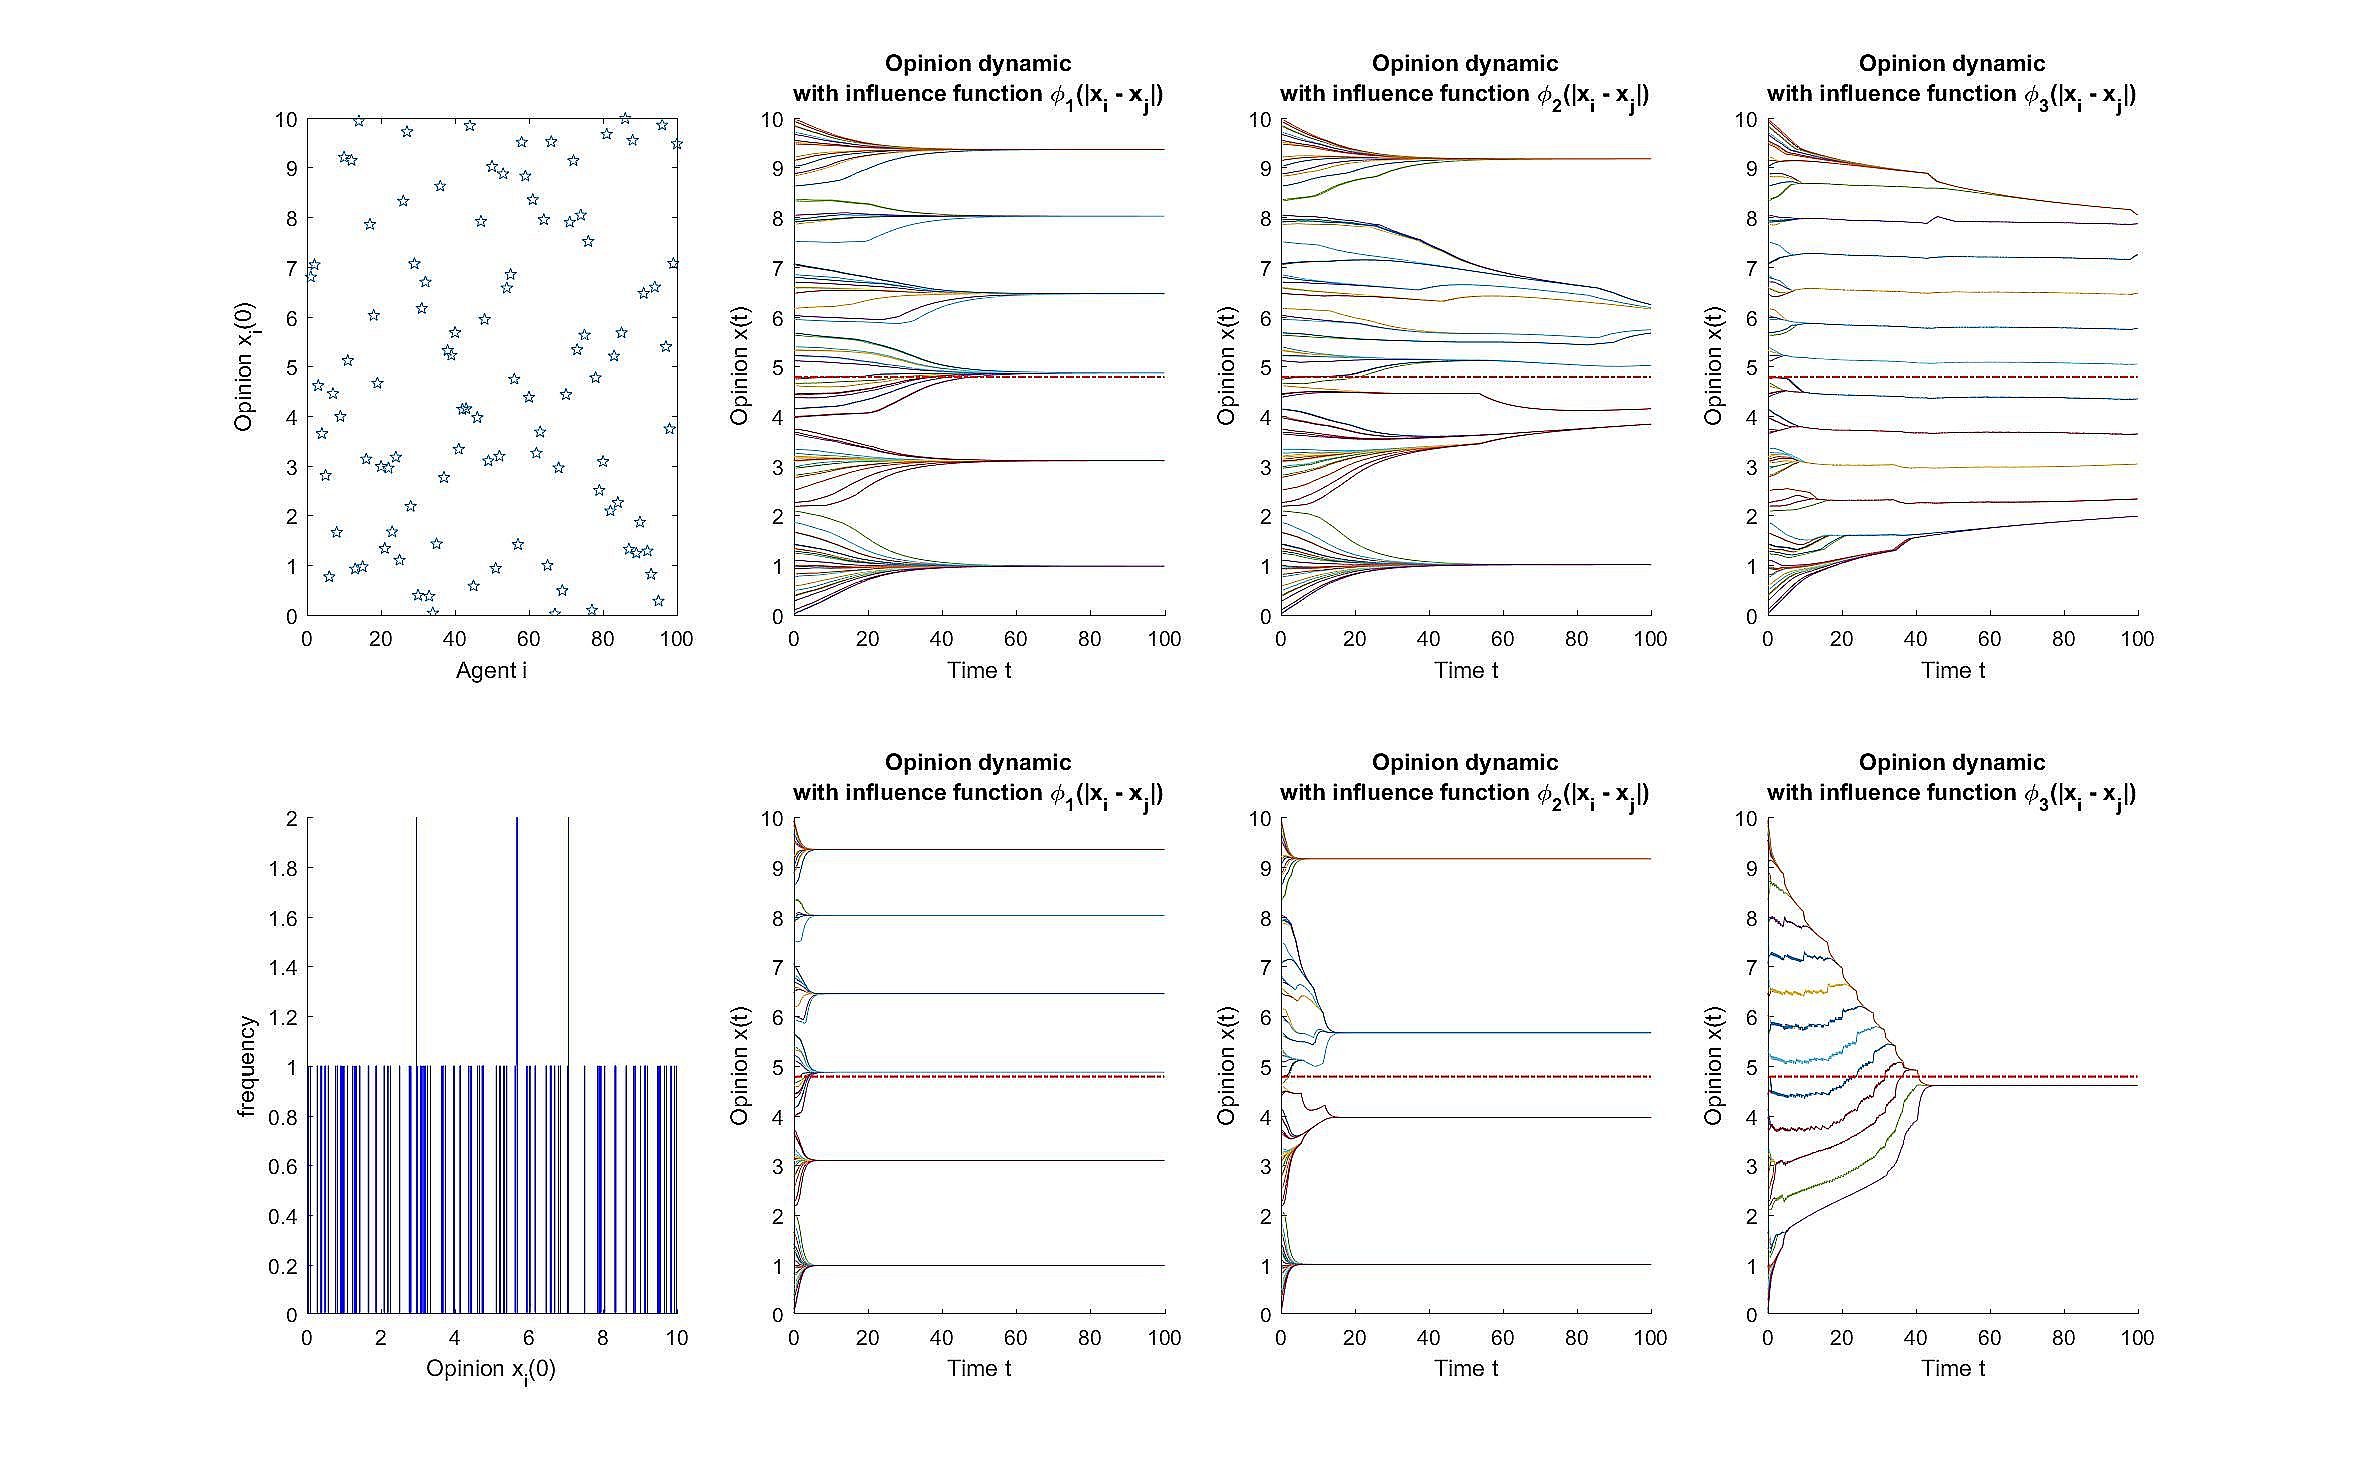
\includegraphics[width=\paperwidth , height=\paperheight]{8}}
\begin{frame}[plain]

\end{frame}
}

{
\usebackgroundtemplate{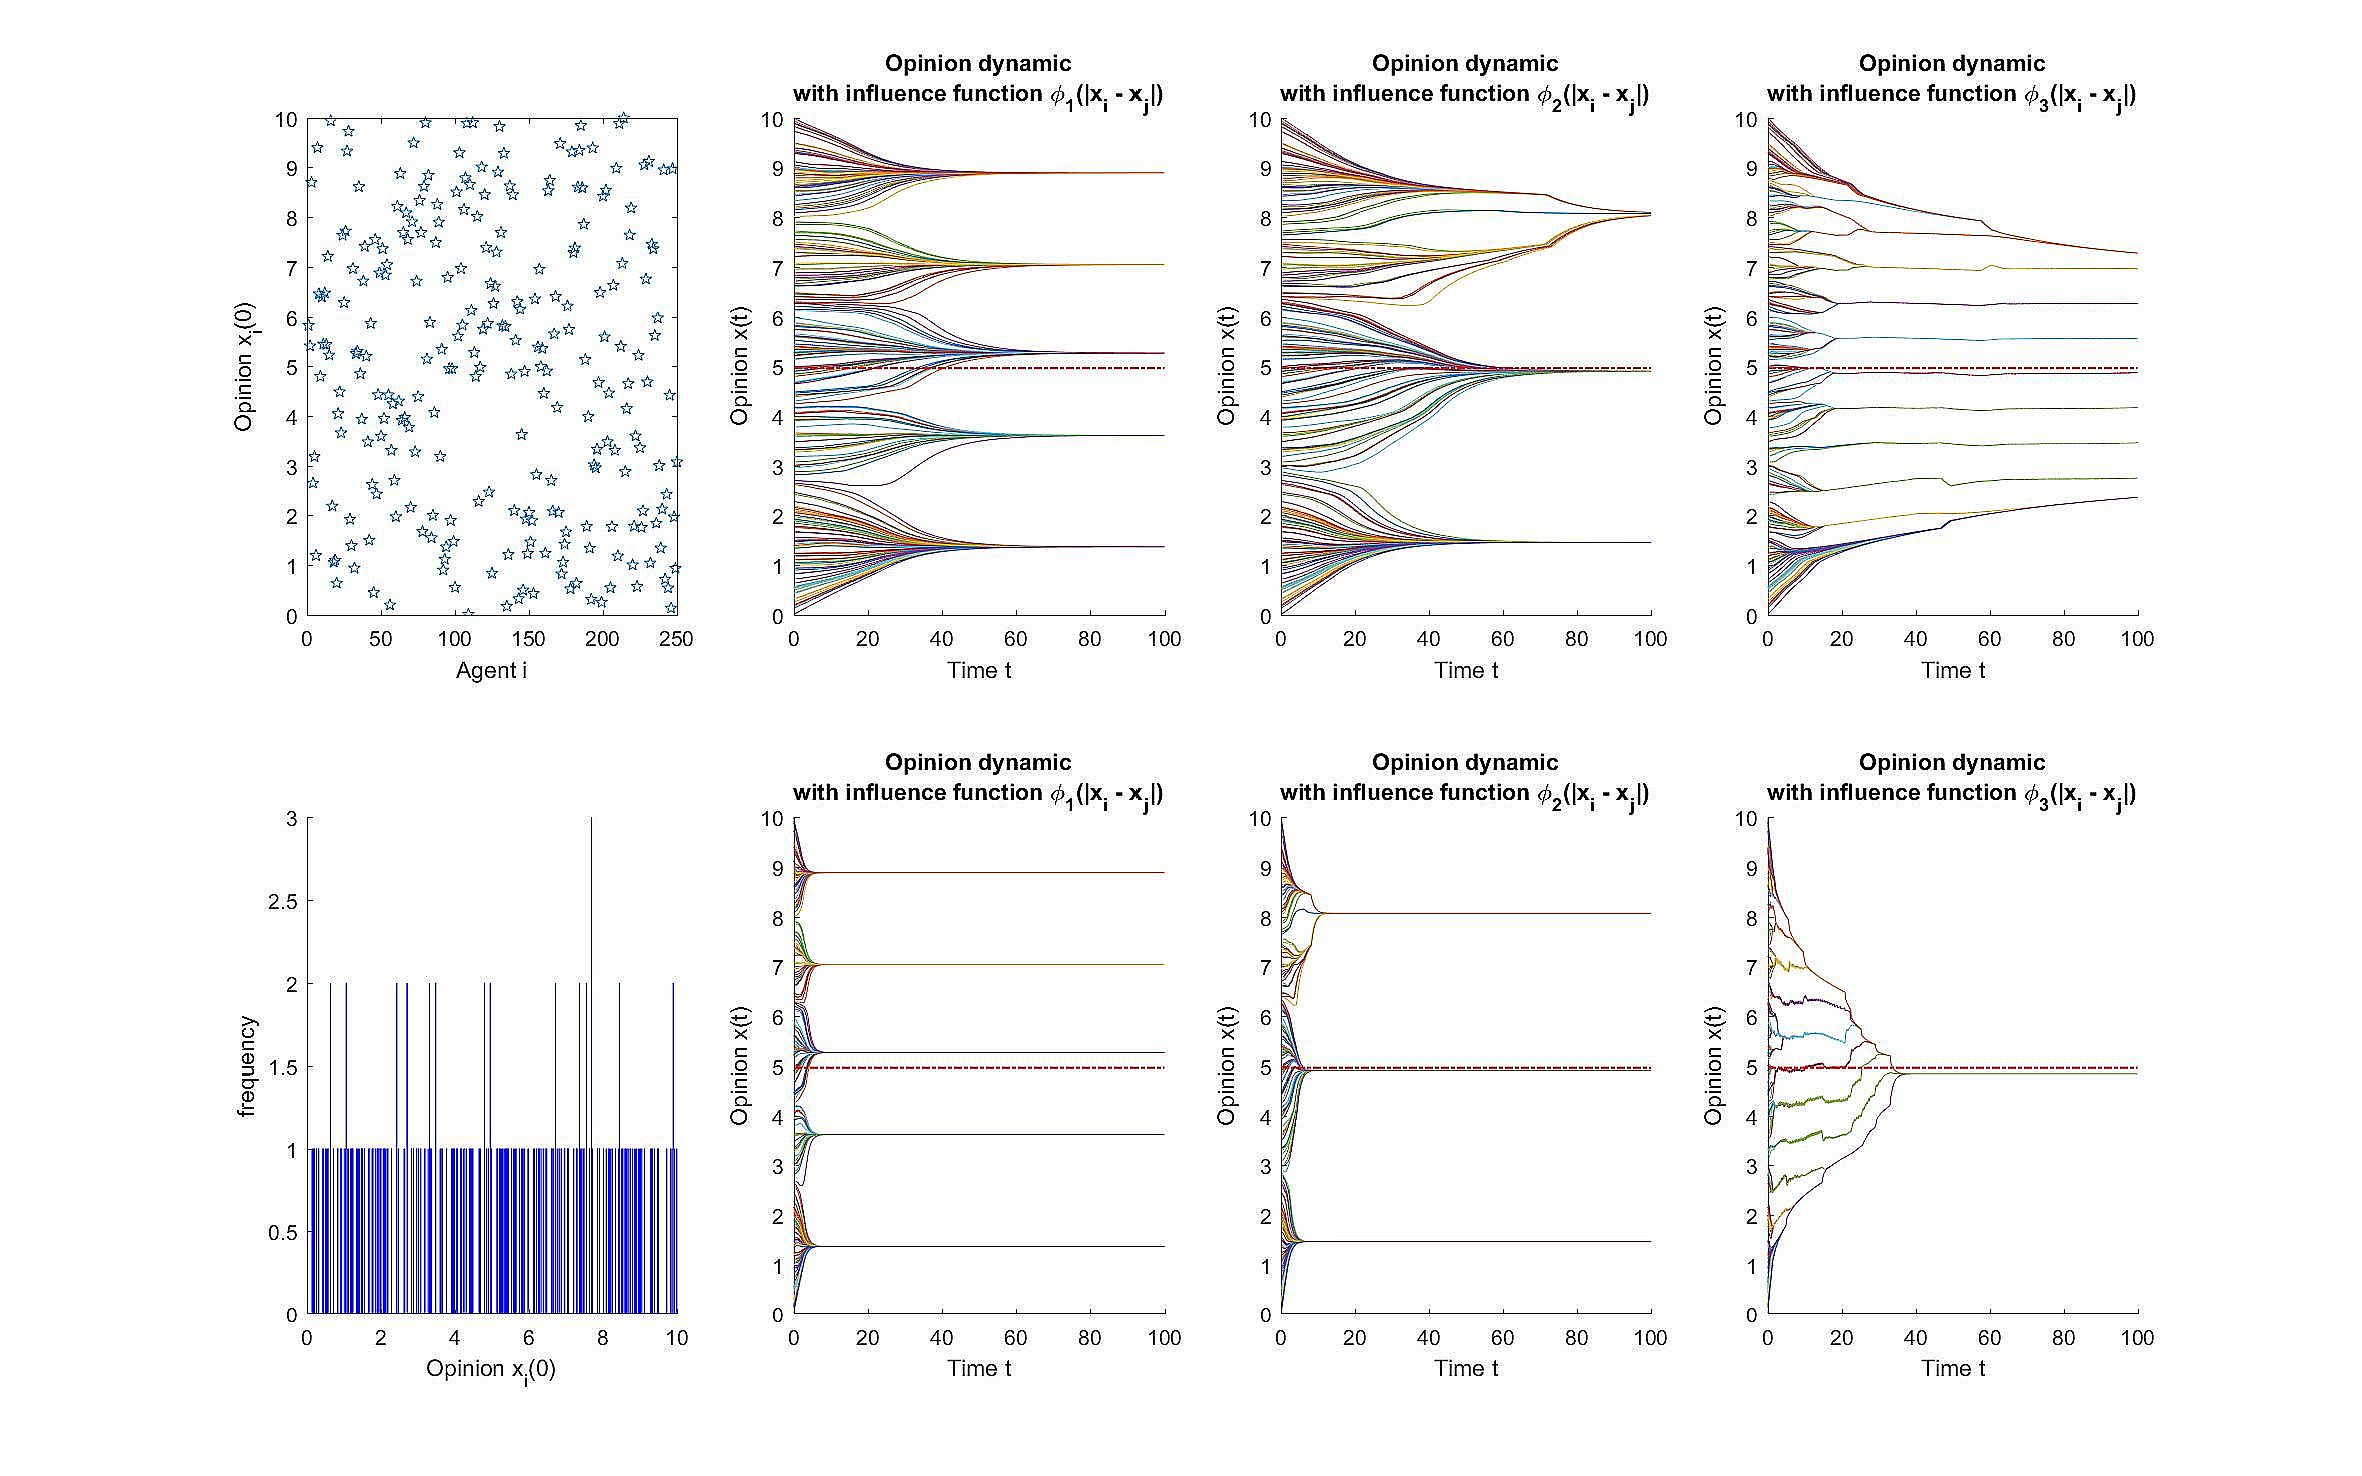
\includegraphics[width=\paperwidth , height=\paperheight]{9}}
\begin{frame}[plain]

\end{frame}
}

\end{document}
